\documentclass[11pt]{article}

\usepackage[letterpaper,top=2cm,bottom=2cm,left=2cm,right=2cm,marginparwidth=1.75cm]{geometry}
\usepackage{hyperref}
\usepackage{biblatex}
\addbibresource{Bib.bib}
\usepackage{mathtools}
\DeclarePairedDelimiterXPP\BigOSI[2]%
  {\mathcal{O}}{(}{)}{}%
  {\SI{#1}{#2}}
\usepackage{xcolor}
\usepackage{empheq}
\usepackage[most]{tcolorbox}
\usepackage{amsmath}
\usepackage{amssymb}
\usepackage{mathrsfs}
\usepackage[utf8]{inputenc}
\usepackage{graphicx}
\usepackage{float}
\usepackage{parskip}
\usepackage{comment}
\usepackage{mhchem}
 \usepackage{tabularx}
 \usepackage{titling}
 \usepackage{amsmath,environ}
 \usepackage[explicit]{titlesec}
\usepackage{fancyhdr}
\usepackage{braket}
\setlength{\droptitle}{3em} 

\title{Quantum Mechanics II}
\author{Thomas Brosnan}
\date{Notes taken in Professor Michael Peardon, Hilary Term 2024}


\newtcbox{\mymath}[1][]{%
    nobeforeafter, math upper, tcbox raise base,
    enhanced, colframe=blue!30!black,
    colback=blue!30, boxrule=1pt,
    #1}
\tcbset{highlight math style={boxsep=2mm,,colback=blue!0!green!0!red!0!}}

  \newenvironment{bux}
    {
    \empheq[box=\tcbhighmath]{align}
   }{
    \endempheq
    }
    \newenvironment{bux*}
    {
    \empheq[box=\tcbhighmath]{align*}
   }{
    \endempheq
    }
\newcommand{\hsp}{\hspace{8pt}}

\newcommand*{\sectionFont}{%
  \LARGE\bfseries
}

    
\numberwithin{equation}{section}

\makeatletter
\let\Title\@title % Copy the title to a new command
\makeatother

%change this RGB value to change the section background colour 
\definecolor{mycolor1}{RGB}{255, 128, 128}
\colorlet{SectionColour}{mycolor1}
%subsection background colour 
\definecolor{mycolor2}{gray}{0.8}
\colorlet{subSectionColour}{mycolor2}
%subsubsection background colour 
\definecolor{mycolor3}{RGB}{255,255,255}
\colorlet{subsubSectionColour}{mycolor3}


\begin{document}

\maketitle

\newpage
\topskip0pt
\vspace*{\fill}
\begin{center}
\Large
    " I am the one who knocks "
    
    - Heisenberg
\end{center}
\vspace*{\fill}
\newpage 
\tableofcontents
% For \section
 \titleformat{\section}[block]{\sectionFont}{}{0pt}{%
 \fcolorbox{black}{SectionColour}{\noindent\begin{minipage}{\dimexpr\textwidth-2\fboxsep-2\fboxrule\relax}\thesection  \hsp #1 {\strut} \end{minipage}}}
% For \subsection
 \titleformat{\subsection}[block]{\bfseries}{}{0pt}{%
 \fcolorbox{black}{subSectionColour}{\noindent\begin{minipage}{\dimexpr\textwidth-2\fboxsep-2\fboxrule\relax}\thesubsection  \hsp #1 {\strut} \end{minipage}}}
% For \section*
 \titleformat{name=\section, numberless}[block]{\sectionFont}{}{0pt}{%
 \fcolorbox{black}{SectionColour}{\noindent\begin{minipage}{\dimexpr\textwidth-2\fboxsep-2\fboxrule\relax} #1 {\strut} \end{minipage}}}
  % For \subsection*
 \titleformat{name=\subsection, numberless}[block]{\bfseries}{}{0pt}{%
 \fcolorbox{black}{subSectionColour}{\noindent\begin{minipage}{\dimexpr\textwidth-2\fboxsep-2\fboxrule\relax} #1 {\strut} \end{minipage}}}
 % For \subsubsection
 \titleformat{\subsubsection}[block]{\bfseries}{}{0pt}{%
 \fcolorbox{black}{subsubSectionColour}{\noindent\begin{minipage}{15cm}\thesubsubsection \hsp #1 {\strut} \end{minipage}}}
  % For \subsubsection*
 \titleformat{name=\subsubsection, numberless}[block]{\bfseries}{}{0pt}{%
 \fcolorbox{black}{subsubSectionColour}{\noindent\begin{minipage}{15cm} #1 {\strut} \end{minipage}}}
\newpage 
%header 
\pagestyle{fancy}
\fancyhf{} % Clear all header and footer fields
\fancyhead[L]{\Title}
\fancyhead[R]{\nouppercase{\leftmark}}
\fancyfoot[C]{-~\thepage~-}
\renewcommand{\headrulewidth}{1pt}











%starting document 
\normalsize
\newpage
\section{Angular Momentum}
\subsection{3D Schrodinger equation}
\begin{itemize}
    \item In QM the Hamiltonian is written in terms of operators. Momenta becomes $\textbf{p} \rightarrow  -i\hbar\nabla $ and the potential $V \rightarrow \hat{V}$ also an operator. So the Hamiltonian becomes:
\begin{bux}
    \begin{split}
        \frac{-\hbar^2}{2m}\nabla^2 + \hat{V}
    \end{split}
\end{bux}
\item The (time independent) Schrodinger equation is: 
\begin{bux}
    \begin{split}
        H \psi(x,y,z) = E \psi
    \end{split}
\end{bux}
\item If we then have a central potential, that is $V=V(r)$, so rotation symmetry generated by a rotational group, we find it best to change co-ords to spherical co-ords. Here the Laplacian is:
\begin{bux}
    \begin{split}
          \nabla^2 = \frac{1}{r^2}\frac{\partial}{\partial r}\left(r^2\frac{\partial}{\partial r}\right) + \frac{1}{r^2\sin(\theta)} \frac{\partial}{\partial \theta}(\sin\theta \frac{\partial \Phi}{\partial \theta}) + \frac{1}{r^2\sin^2(\theta)}\frac{\partial ^2 \Phi}{\partial \phi^2}=0
    \end{split}
\end{bux}
We then make the typical assumption of separation of variables, that is:
\begin{bux}
    \begin{split}
        \psi = R(r)Y(\theta,\phi)
    \end{split}
\end{bux}
The Schrodinger equation then becomes: 
\begin{bux}
    \begin{split}
       -  \frac{\hbar^2}{2m}& \left[\frac{Y}{r^2}\frac{\partial}{\partial r}\left(r^2\frac{\partial R}{\partial r}\right)+ \frac{R}{r^2\sin\theta} \frac{\partial}{\partial \theta}(\sin \theta \frac{\partial Y}{\partial \theta}) + \frac{R}{r^2\sin^2 \theta}\frac{\partial ^2Y}{\partial \phi^2}\right] \\
& + V(r)R(r)Y(\theta,\phi) = ER(r)Y(\theta,\phi)
    \end{split}
\end{bux}
Dividing by $R(r)Y(\theta,\phi)$ and multiplying by $r^2$, we get two terms, one a function of $r$ only and one a function of $\theta$ and $\phi$, adding to a constant $E$. This means that both these terms must themselves be constant.  This gives us two separate equations. 
\begin{bux}
    \begin{split}
\label{eqn:1.6}
       &  -  \frac{1}{R}\frac{d}{d r}\left(r^2\frac{d R}{d r}\right) - \frac{2mr^2}{\hbar^2}[V(r)-E] = l(l+1) \\ 
& \frac{1}{Y}\left[ \frac{1}{\sin \theta}\frac{\partial}{\partial \theta}(\sin \theta \frac{\partial  Y}{\partial \theta})+ \frac{1}{\sin^2 \theta}\frac{\partial^2Y}{\partial \phi^2}\right] = -l(l+1)
    \end{split}
\end{bux}
The choice $l(l+1)$ as a constant, may seem strange at first but makes sense later. On the later equation we again perform separation of variables, $Y = \Theta(\theta)\Phi(\phi)$, so we get two more equations: 
\begin{bux}
    \begin{split}
       &  \frac{1}{\Phi}\frac{d^2 \Phi}{d \phi^2} = -m^2 \\
\sin \theta \frac{d}{d \theta}\left( \sin \theta \frac{d \Theta}{d \theta}\right)& + \left(l(l+1)\sin^2 \theta - m^2 \right)\Theta = 0 
    \end{split}
\end{bux}
The first equation here is solved by the usual: 
\begin{bux}
    \begin{split}
    \label{eqn:1.8}
        \Phi \propto e^{\pm i m \phi} 
    \end{split}
\end{bux}
And Linear combinations of this. Since we would expect that $\Phi(\phi+2\pi) = \Phi(\phi) $, as $\phi$ is multi-valued, this sets the restriction on $m$, that $m$ must be an integer. 

The solution to $\Theta$ solved by the \emph{associated Legendre functions} $P^m_l$: 
\begin{bux}
    \begin{split}
\label{eqn:1.9}
        &\Theta \propto  P^m_l(\cos \theta)  \\ 
 P^m_l(x)  =& (1-x^2)^{\frac{|m|}{2}} \left( \frac{d}{dx}\right)^{|m|}P_l(x)
    \end{split}
\end{bux}
Here $P_l(x)$ are the Legendre polynomials, which can be generated from the Rodrigues' formula: 
\begin{bux}
    \begin{split}
          P_l(x) = \frac{1}{2^ll!}\frac{d^l}{dx^l}(x^2-1)^l
    \end{split}
\end{bux}
This generates a polynomial of degree $l$, this means that \ref{eqn:1.9} vanishes if $|m|>l$ as the $n$th derivative of a $(n-1)$th order polynomial is $0$. So we have that: 
\begin{bux}
    \begin{split}
        & |m|\leq l \\ 
\implies m \in  \{ &-l,...,0,...,l \}
    \end{split}
\end{bux}
There are $2l+1$ allowed values for $m$. Because the Radial equation \ref{eqn:1.6}, does not contain $m$ but does depend on $l$. We get degenerate solutions as the only restriction is $|m|\leq l$. This leads to degenerate solutions due to symmetry.  
\end{itemize}

\subsection{Spherical Harmonics}
\begin{itemize}
    \item With the above equations we can now calculate the form of $Y^m_l(\theta,\phi) = \Theta(\theta)\Phi(\phi)$, these functions are known as the spherical harmonics.  The first harmonic $Y^0_0$ is just a constant, It can be of any form to satisfy the  differential equation set for $Y$, but we usually specify it so that the wavefunction is normalised. This turns out to set: 
\begin{bux}
    \begin{split}
        Y^0_0 = \sqrt{\frac{1}{4\pi}}
    \end{split}
\end{bux}
\item In a similar manner the prefactor for the constant in front of any $Y^m_l(\theta, \phi)$ can be calculated. This allows us to then write out the full form of the $Y^m_l(\theta, \phi)$ functions using \ref{eqn:1.8} and \ref{eqn:1.9}: 
\begin{bux}
    \begin{split}
\label{eqn:1.14}
        Y_l^m = (-1)^{m}\sqrt{\frac{2l+1}{4\pi}\frac{(l-m)!}{(l+m)!}} P_l^{m}(\cos \theta)e^{im\phi}
    \end{split}
\end{bux}
There is only one harmonic for $l=0 \implies m=0$ , but for $l=1, m \in \{-1,0,1\}$, so there are three harmonics: 
\begin{bux}
    \begin{split}
        Y^{-1}_1 = \sqrt{\frac{3}{8\pi}}\sin \theta e^{-i\phi},~~~Y^{0}_1 = \sqrt{\frac{3}{4\pi}}\cos \theta,~~~Y^{1}_1 = \sqrt{\frac{3}{8\pi}}\sin \theta e^{i\phi}
    \end{split}
\end{bux}
\item We can realise some cool things if we notice how these relate to the standard conversion from Cartesian to spherical co-ords, given by: 
\begin{bux}
    \begin{split}
        & x_1 = r \sin \theta \cos \phi \\ 
&  x_2 =  r \sin \theta \sin \phi \\ 
& x_3 = r\cos  \theta 
    \end{split}
\end{bux}
We can construct three new functions $\tilde{Y}^{\alpha}_1, \alpha = 1,2,3$, where: 
\begin{bux}
    \begin{split}
         & \tilde{Y}_1^3 \equiv Y^0_1 =  \sqrt{\frac{3}{4 \pi}}\frac{x_3}{r} \\ 
  \tilde{Y}_1^1 &=  \frac{1}{\sqrt{2}}(Y^{-1}_1-Y^1_1) = \sqrt{\frac{3}{4 \pi }}\frac{x_1}{r} \\ 
 \tilde{Y}_1^2& =  \frac{1}{\sqrt{2}}(Y^{-1}_1+Y^1_1) = \sqrt{\frac{3}{4 \pi }}\frac{x_2}{r}
    \end{split}
\end{bux}
If we rotate around the origin by an angle $\gamma$ then $\textbf{x}$ transforms by:
\begin{bux}
    \begin{split}
        \textbf{x}' = \Lambda(\gamma)\textbf{x}
    \end{split}
\end{bux}
Where $\Lambda$ is just a rotation matrix. It can then be seen that the by the form of the three $Y_1^{\alpha}$, that they transform the same way (as $r$ remains constant). They are like the components of the vector $\tilde{\textbf{Y}}$, with: 
\begin{bux}
    \begin{split}
        \tilde{\textbf{Y}}' = \Lambda(\gamma)\tilde{\textbf{Y}}
    \end{split}
\end{bux}
These $\tilde{Y}_1^{\alpha}$ form a representation of the group of rotations. When $l=2$ this becomes a tensor representation. 
\item We can combine $Y^m_l$ in combinations to form others. Take for instance $Y^0_2$ given by: 
\begin{bux}
    \begin{split}
        Y^0_2 = \sqrt{\frac{5}{16 \pi}}(3 z\cos^2 \theta -1)
    \end{split}
\end{bux}
From examining the above expressions we can see that this must be related to $(Y^0_1)^2= \frac{3}{4}\cos^2 \theta $. In fact we can write $Y_1^0$ in terms of $Y_2^0$, where we can take care of any constant term by writing it in terms of $Y_0^0$. This takes the form: 
\begin{bux}
    \begin{split}
        (Y_1^0)^2 = \frac{1}{\sqrt{4 \pi }} (Y_0^0+ \frac{2}{\sqrt{5}} Y_2^0)
    \end{split}
\end{bux}
It can be noted that for $m$'s the two sides add, $0+0 =0+0$, and $l$'s $1+1=0+2$. This becomes important later on. 
\end{itemize}

 \subsection{Angular Momentum operators} 
 \begin{itemize}
     \item Classically angular momentum is defined as $\textbf{L} = \textbf{p}\times\textbf{x} $. In quantum mechanics $P_k \rightarrow -i\hbar \frac{\partial}{\partial x_k}$. So the angular momentum operators are: 
\begin{bux}
    \begin{split}
        & \hat{L}_1 = - i \hbar(x_2\frac{\partial}{\partial x_3} - x_3\frac{\partial}{\partial x_2}) \\ 
&\hat{L}_2 = - i \hbar(x_2\frac{\partial}{\partial x_3} - x_3\frac{\partial}{\partial x_2}) \\ 
&\hat{L}_3 = - i \hbar(x_2\frac{\partial}{\partial x_3} - x_3\frac{\partial}{\partial x_2})
    \end{split}
\end{bux}
These have the useful property that $[\hat{L}_{\alpha},L_{\beta}] = i \hbar \epsilon_{\alpha \beta \gamma} \hat{L}_{\gamma}$
\item We also define the total angular momentum operator as: 
\begin{bux}
    \begin{split}
        \hat{L}^2 = \hat{L}_1^2 + \hat{L}_2^2 + \hat{L}_3^2
    \end{split}
\end{bux}
This has the property that, $[\hat{L}^2,\hat{L}_k] =0 $, for all $k=1,2,3$. 
\item We can see how the angular momentum operators $\hat{L}_{\alpha}$ act on the the $Y_m^l$ functions if we convert them into polar co-ords.  This is a tedious process but the results are: 
\begin{bux}
    \begin{split}
         \hat{L}_1 =  i\hbar(&\sin \phi \frac{\partial}{\partial \theta} - \cot \theta \cos \phi \frac{\partial }{\partial \phi}) \\
  \hat{L}_2 =   -i\hbar(&\cos \phi \frac{\partial}{\partial \theta} - \cot \theta \sin \phi \frac{\partial }{\partial \phi})  \\
& \hat{L}_3  = -i\hbar \frac{\partial}{\partial \phi}
    \end{split}
\end{bux}
\item We can also calculate the expression for the total angular momentum operator: 
\begin{bux}
    \begin{split}
        \hat{L}^2 = -\hbar^2\left(\frac{1}{\sin \theta}\frac{\partial}{\partial \theta}(\sin\theta\frac{\partial}{\partial \theta}) + \frac{1}{\sin^2\theta}\frac{\partial^2}{\partial \phi^2} \right)
    \end{split}
\end{bux}
\item Acting with $\hat{L}^2$ on our state $\ket{l,m} = Y_l^m(\theta,\phi)$ given by \ref{eqn:1.14}, we get the same equation we had for the spherical harmonics in the first place  \ref{eqn:1.6}, with a prefactor!  So we can say:
\begin{bux}
    \begin{split}
        \hat{L}^2\ket{l,m} = \hbar^2l(l+1)\ket{l,m}
    \end{split}
\end{bux}
We can also see that acting on $\ket{l,m}$ with $\hat{L}_3$ leads to:
\begin{bux}
    \begin{split}
        \hat{L}_3\ket{l,m} = \hbar m\ket{l,m}
    \end{split}
\end{bux}
Thus we can see these $Y_l^m$'s are eigenstates of the total angular momentum and the angular momentum in the $z$ direction. 
 \end{itemize}
    \subsubsection{Ladder operators}
    \begin{itemize}
        \item The following operators are defined for the $z$-axis having the eigenvalue $m$, i.e. the angle $\phi$ rotates around the $z$-axis. If this was different the below operators would be too. We define the following two operators, known as the ladder operators: 
\begin{bux}
    \begin{split}
        \hat{L}_{\pm} = \hat{L}_1 \pm i\hat{L}_2
    \end{split}
\end{bux}
These are often used instead of $\hat{L}_1$ and $\hat{L}_2$ as the commutators with $\hat{L}^2$ and $\hat{L}_3$ are:
\begin{bux}
    \begin{split}
        [\hat{L}_3,\hat{L}_{\pm}] = i\hbar\hat{L}_{\pm} , ~~~ [\hat{L}^2,\hat{L}_{\pm}] = 0 
    \end{split}
\end{bux}
The first result means if some state $\ket{l,m}$ is an eigenstate of $\hat{L^2},\hat{L}_3$, then so is $\hat{L}_{\pm}\ket{l,m}$. This can be seen from the following: 
\begin{bux}
    \begin{split}
        \hat{L}_3\hat{L}_{\pm}\ket{l,m} = (\pm\hbar\hat{L}_{\pm}+\hat{L}_{\pm}\hat{L}_3)\ket{l,m} = \hbar(m\pm1)\hat{L}_{\pm}\ket{l,m}
    \end{split}
\end{bux}
It can also be shown that the ladder operators act in the following way on the kets $\ket{l,m}$: 
\begin{bux}
    \begin{split}
\label{eqn:1.30}
       &  \hat{L}_{-}\ket{l,m} = \hbar\sqrt{l(l+1)-m(m-1)}\ket{l,m-1} \\ 
      & \hat{L}_+\ket{l,m} = \hbar\sqrt{l(l+1)-m(m+1)}\ket{l,m+1}
    \end{split}
\end{bux}
This is why they are called ladder operators, they cycle through the eigenvalues of $\hat{L}_3$. 
    \end{itemize}
\subsubsection{Total angular momentum eigenvalue}
\begin{itemize}
    \item It is not quite clear why $l(l+1)$ is the eigenvalue of the total angular momentum. To see why this is the case we simply have to construct the following argument.  Using the above definitions of the ladder operators it can be shown that the total angular momentum operator $\hat{L}^2$ can be expressed as: 
\begin{bux}
    \begin{split}
         \hat{L}^2 = \hat{L}_1^2 + \hat{L}_2^2 + \hat{L}_3^2 = \hat{L}_-\hat{L}_++ \hat{L}_3^2+\hat{L}_3
    \end{split}
\end{bux}
So if we consider a state with the maximum angular momentum in the $z$-direction then we have that the state is $\ket{l,l}$.  We then know that $\hat{L}_+\ket{l,l} = 0 $ and $\hat{L}_3\ket{l,l} = l\ket{l,l}$, so if we want to find the expected total angular momentum $\braket{\hat{L}^2} = \bra{l,l}\hat{L}^2\ket{l,l}$: 
\begin{bux}
    \begin{split}
        \braket{\hat{L}^2} = \bra{l,l}\hat{L}_-\hat{L}_++ \hat{L}_3^2+\hat{L}_3\ket{l,l} = \bra{l,l}(l^2+l)\ket{l,l} = l(l+1)
    \end{split}
\end{bux}
As needed. 
\end{itemize}
\subsection{Two particle system}
\begin{itemize}
    \item For a system of two particles there are two ways of looking at it. First we can consider the two particles $a$ and $b$. Then they have separate states with separate quantum numbers, $\ket{l^{(a)},m^{(a)}}$ and $\ket{l^{(b)},m^{(b)}}$ and the total state $\ket{l^{(a)},m^{(a)};l^{(b)},m^{(b)}}$ The total angular momentum operators for the system then look like: 
\begin{bux}
    \begin{split}
        \hat{L}_k^{(\text{total})} &= \hat{L}_k^{(a)} +\hat{L}_k^{(b)},~~~k=1,2,3 \\ 
     & \hat{L}_{(total)}^2  = \sum_{k=1}^3\left(\hat{L}_k^{(\text{total})}\right)^2
    \end{split}
\end{bux}
Another way is to look at this system is as one state $\ket{l^{(total)},m^{(total)}}\equiv \ket{l,m}$, a different basis. The problem with this then is that an eigenstate $\ket{l,m}$ of $\hat{L}^{(total)^2}$ will not be an eigenstate of $\hat{L}^2_{(a)}$ or $\hat{L}^2_{(b)}$ as $ \hat{L}_{(\rm total)}^2  = \sum_{k=1}^3(\hat{L}_k^{(a)} +\hat{L}_k^{(b)})^2$, which is not linear. 

We wish to be able to "connect" these two descriptions of the same system. To do this we consider the simplest case, two particles each with the minimum total angular momentum $\hbar \implies l=1$, there are then $2l+1=3$ possible particles states for each particle. So the possible combined states of the two particles are as follows: 
\begin{bux}
    \begin{split}
       & \ket{1,-1;1,-1}, \ket{1,-1;1,0}, \ket{1,-1;1,1} \\
       & \ket{1,0;1,-1}, ~~~\ket{1,0;1,0}, ~~~\ket{1,0;1,1} \\
       & \ket{1,1;1,-1}, ~~~\ket{1,1;1,0}, ~~~\ket{1,1;1,1}
    \end{split}
\end{bux}
\item We then want to look at the system as a whole, we know the maximum total angular momentum is $2l=2$ and that the angular momentum in the $z$-direction will vary from $M=-2,-1,0,1,2$. Unlike total angular momentum this is just the sum total of the two z-components of the particles, $M = m^{(a)}+m^{(b)}$,   Each value of $M$ can have more then one possible configuration of the two particles, to find these states and their normalization's we can use the ladder operators. 

\item For the highest value of $M$ there is only one configuration: 
\begin{bux}
    \begin{split}
        \ket{2,2} = \ket{1,1;1,1}
    \end{split}
\end{bux}
To find $\ket{2,1}$ we can act on the LHS with $\hat{L}_-^{(\rm total)}$ and on the RHS with the two particle form $\hat{L}_-^{(a)}+\hat{L}_-^{(b)}$, these act on these kets according to \ref{eqn:1.30}. These operators also only act on the respective parts of the kets as is shown: 
\begin{bux}
    \begin{split}
        & \hat{L}_-^{(\rm total)}\ket{2,2} = \hat{L}_-^{(a)} \ket{1,1;1,1}+\hat{L}_-^{(b)}\ket{1,1;1,1} \\ 
&  2\hbar\ket{2,1} = \sqrt{2}\hbar\ket{1,0;1,1} + \sqrt{2}\hbar\ket{1,1;1,0} \\
\implies&  \ket{2,1} = \frac{1}{\sqrt{2}}  \ket{1,0;1,1} + \frac{1}{\sqrt{2}}\ket{1,1;1,0}
    \end{split}
\end{bux}
\item We can then just repeat this to get $\ket{2,0}$ and $\ket{2,-1}$. $\ket{2,-2}$ is again just one state.  The results of these are: 
\begin{bux}
    \begin{split}
        \ket{2,0} =& \frac{1}{\sqrt{6}}\ket{1,-1;1,1} + \frac{2}{\sqrt{6}}\ket{1,0;1,0} + \frac{1}{\sqrt{6}}\ket{1,1;1,-1} \\ 
 &  \ket{2,-1} =\frac{1}{\sqrt{2}}\ket{1,0;1,-1} + \frac{1}{\sqrt{2}}\ket{1,-1;1,0} \\
& \ket{2,-2} = \ket{1,-1;1,-1}
    \end{split}
\end{bux}
The only problem with this is that it misses the states with $l=1$ or  $l=0$.  To solve this we look at the states of $a$ and $b$ that we know $\ket{1,1}$ must be made of: 
\begin{bux}
    \begin{split}
        \ket{1,1} = \alpha\ket{1,1;1,0} + \beta \ket{1,0;1,1}
    \end{split}
\end{bux}
This state must be normalised so $|\alpha|^2+|\beta|^2=1$ and it must be orthogonal to the other states, so we can use $\braket{2,1|1,1}=0$. This tells us $\frac{1}{\sqrt{2}}\beta + \frac{1}{\sqrt{2}}\alpha = 0 \implies \alpha = -\beta$. These constraints can be solved to get $\alpha =\frac{1}{\sqrt{2}}$ and $\beta = -\frac{1}{\sqrt{2}}$, so we can write:
\begin{bux}
    \begin{split}
        \ket{1,1} = \frac{1}{\sqrt{2}}\ket{1,1;1,0} -  \frac{1}{\sqrt{2}}\ket{1,0;1,1}
    \end{split}
\end{bux}
\item To get $\ket{1,0}$ and $\ket{1,-1}$ we can just do the same process of acting with $\hat{L}_-^{(total)}$. The results are: 
\begin{bux}
    \begin{split}
       &   \ket{1,0} = \frac{1}{\sqrt{2}}\ket{1,1;1,-1} -  \frac{1}{\sqrt{2}}\ket{1,-1;1,1} \\
& \ket{1,-1} = \frac{1}{\sqrt{2}}\ket{1,-1;1,0} -  \frac{1}{\sqrt{2}}\ket{1,-1;1,1} 
    \end{split}
\end{bux}
We repeat this one more to find the last state $\ket{0,0}$. This must be a linear combination of the final three states 
and we can solve for the co-officiants by making sure it is orthogonal to $\ket{1,0}$ and $\ket{2,0}$. The result of this is:
\begin{bux}
    \begin{split}
        \ket{0,0} = \frac{1}{\sqrt{3}}\left(\ket{1,1;1,-1}  -\ket{1,0;1,0} + \ket{1,-1;1,1}   \right)
    \end{split}
\end{bux}
\end{itemize}

\subsection{Half-integer-spin}
\begin{itemize}
    \item All though we derived through the construction of the $Y_l^m$'s that $l$ and $m$ must be integer values, the mathematics describing angular momentum using the angular momentum operators, works just fine if $l$ can take on half integer values. $m$ can still satisfy $m \in  \{ -l,...,0,...,l \}$, and is thus also a half integer. before there were $2l+1$ possible values of $m$ with $l$ being an integer, so always an odd amount. But now with $l$ a half integer, there are always an even number of possible $m$ values and notably $m$ can never be $0$, as it is not a half integer. 
\end{itemize}


\subsection{Clebsch-Gordan coefficients}
\begin{itemize}
    \item The coefficients in front of each two particle state, when making up the state of the single particle system are what we call the Clebsch-Gordan coefficients. These are the prefactors we saw in the above example. They will look different for two particles with spin $\neq 1$. A table showing all the values is shown below: 
\end{itemize}


\begin{figure}[H]
\centering
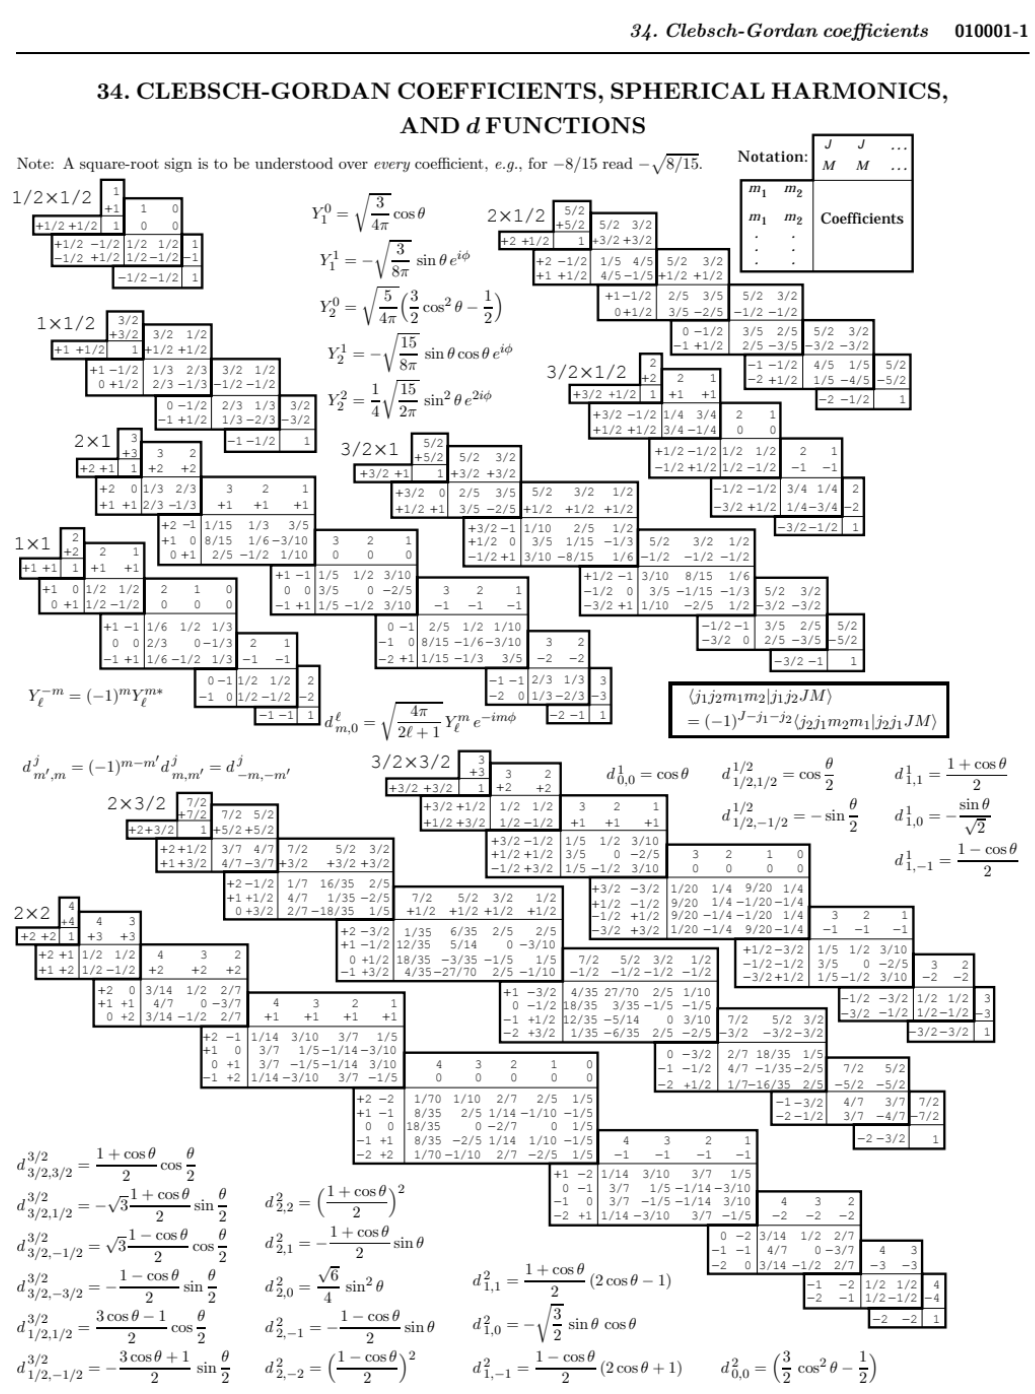
\includegraphics[width=0.9\textwidth]{image.png}
\caption{\label{fig:2}\small \emph{The sign convention is that of Wigner (Group Theory, Academic Press, New York, 1959), also used by Condon and Shortley (The Theory of Atomic Spectra, Cambridge Univ. Press, New York, 1953), Rose (Elementary Theory of Angular Momentum, Wiley, New York, 1957),and Cohen (Tables of the Clebsch-Gordan Coefficients, North American Rockwell Science Center, Thousand Oaks, Calif., 1974). The coefficients here have been calculated using computer programs written independently by Cohen and at LBNL .}}
\end{figure}

\begin{itemize}
    \item As can be seen from the $1 \times 1$ (by this we mean two particles of spin $\hbar$), the only possible total angular momentum values we found were $l=0,1,2$ . We would like to generalise this and see what types of total angular momentum can we see from two particles with individual total angular momentum $l_1$ and $l_2$ .  It can be seen that however many different values of $l$ there are they will always be spaced 1 apart, this can be seen from the fact that if we have the maximum value of $l$, i.e. $l=l_1+l_2$ then the next lowest value will be $l=l_1+l_2-1$. 

\item The problem is then finding how low to go. For this we can impose that the two views of the system (one as a two particle system and one as a single particle system) must have the same number of possible $L_3$ states. For the two particle states this is simple, it is just the product of the number of values of $m_1$ and $m_2$, so $(2l_1+1)(2l_2+1)$. Where as for the two particle system, the total number of states will be the sum of $(2l+1)$ for all the possible values of $l$. We only know the largest value of $l$ that being $l_1+l_2$, and we will call the lowest value $a$. This means are condition of equal number of states takes the form: 
\begin{bux}
    \begin{split}
        \sum_{l=a}^{l_1+l_2}(2l+1) = (2l_1+1)(2l_2+1)
    \end{split}
\end{bux}
We can then re-write this sum using $l=a+n$ so that $a=l \implies n=0$. This means: 
\begin{bux}
    \begin{split}
          \sum_{l=a}^{l_1+l_2}(2l+1) =&    \sum_{n=0}^{l_1+l_2-a}(2(a+n)+1) = (2a+1)(l_1+l_2-a+1) + 2\sum_{n=0}^{l_1+l_2-a}n \\
=&   (2a+1)(l_1+l_2-a+1) + (l_1+l_2-a)(l_1+l_2-a+1) \\
=& (l_1+l_2+a+1)(l_1+l_2-a+1) \\
=& l_1^2 +2l_1l_2+2l_1+2l_2+l_2^2-a^2+1
    \end{split}
\end{bux}
Now we know this must be equal to $(2l_1+1)(2l_2+1) = 4l_1l_2+2l_1+2l_2+1$. So the condition on $a$ is that: 
\begin{bux}
    \begin{split}
       &  l_1^2-2l_1l_2 +l_2^2 - a^2=0 \\ 
 & \implies a^2 =(l_1-l_2)^2 \\ 
& \implies   a = |l_1-l_2|
    \end{split}
\end{bux}
A consequence of this is that $|l_1-l_2|\geq 0$, which is expected, with $|l_1-l_2|\neq 0$ if the two particles have different total angular momentum values. This is understandable as we would expect them to never be able to fully cancel out.  

\item We can write this down concisely in the form of Hilbert spaces. Mathematically this different way of viewing the same system is equivalent to decomposing the Hilbert spaces into the direct product of irreducible representations. This is written as: 
\begin{bux}
    \begin{split}
       \mathcal{H}_{l_1} \otimes \mathcal{H}_{l_2} = \mathcal{H}_{l_1+l_2} \oplus  \mathcal{H}_{l_1+l_2-1}\oplus \cdot \cdot \cdot \oplus \mathcal{H}_{|l_1-l_2|}
    \end{split}
\end{bux}
\item The LHS being a product corresponds to how the two particles are both in different states. Where as the RHS being a sum of different Hilbert spaces, corresponds to how the system looks like it is one particle with total angular momentum $l_1+l_2$ or $l_1+l_2-1$ or $\cdot \cdot \cdot$ etc. 

 \end{itemize}

\newpage
\section{Two particle Wave functions}
\begin{itemize}
    \item Here we will be dealing with the time independent Schr\"odinger equation (TISE). We will write down the composite wave function as:  $\Psi(\textbf{x}_1,\textbf{x}_2)$. This means the full wavefunction takes the form: 
\
\begin{bux}
    \begin{split}
        \left[-\frac{\hbar^2}{2}\left( \frac{1}{m_1}\nabla^2_1 + \frac{1}{m_2}\nabla^2_2\right) +V(\textbf{x}_1,\textbf{x}_2)\right]\Psi = E\Psi
    \end{split}
\end{bux}
This wavefunction is a square integrable function, so it forms a continuous probability density. This means: 
\begin{bux}
    \begin{split}
        |\Psi(\textbf{x}_1,\textbf{x}_2)|^2d^3x_1d^3x_2
    \end{split}
\end{bux}
Is the probability $\textbf{x}_1$ lies in the volume $d^3x_1$ and $\textbf{x}_2$ lies in $d^3x_2$.  Being square integrable the we can normalize this wavefunction so that: 
\begin{bux}
    \begin{split}
          \int\int |\Psi(\textbf{x}_1,\textbf{x}_2)|^2d^3x_1d^3x_2 =1
    \end{split}
\end{bux}
\end{itemize}
\subsubsection{Non-interacting particles }
\begin{itemize}
    \item Non-interacting particles mean the potential can be split up into $V(\textbf{x}_1,\textbf{x}_2) = V_1(\textbf{x}_1)+ V_2(\textbf{x}_2)$. This makes it possible to separate the wave function as an ansatz so that $\Psi(\textbf{x}_1,\textbf{x}_2) = \psi_1(\textbf{x}_1)\psi_2(\textbf{x}_2)$. This makes it so that the Schr\"odinger equation splits up into two separate equations :
\begin{bux}
    \begin{split}
         &  -\frac{\hbar^2}{2m_1}\frac{1}{\psi_1} \nabla^2_1 \psi_1+V_1(\textbf{x}_1)-E_1\\
& -\frac{\hbar^2}{2m_2}\frac{1}{\psi_2}\nabla^2_2\psi_2+V_2(\textbf{x}_2)-E_2 = 0
    \end{split}
\end{bux}
\end{itemize}
\subsubsection{Two interacting particles }
\begin{itemize}
    \item If we have two interacting particles, then $V(\textbf{x}_1,\textbf{x}_2) = V(|\textbf{x}_1-\textbf{x}_2|)$. Now to solve the Schr\"odinger equation it makes sense to change to relative ($\textbf{d} = \textbf{x}_1-\textbf{x}_2$) and center of mass coordinates $\textbf{q} = \frac{m_1\textbf{x}_1+m_2\textbf{x}_2}{m_1+m_2}$. This is a linear transformation and can be concisely put with: 
\begin{bux}
    \begin{split}
        \begin{pmatrix}
            \textbf{d} \\
            \textbf{p}
        \end{pmatrix} = \begin{pmatrix}
            1 & -1 \\
            \frac{m_1}{m_1+m_2)} & \frac{m_2}{m_1+m_2)}
        \end{pmatrix}\begin{pmatrix}
            \textbf{x}_1 \\
            \textbf{x}_2
        \end{pmatrix}
    \end{split}
\end{bux}
This way $\rm det(J)=1$, where $J$ is this transformation matrix. This change of co-ords means the Schr\"odinger equations takes the form: 
\begin{bux}
    \begin{split}
        \left[-\frac{\hbar^2}{2\mu}\left( \nabla^2_d + \nabla^2_q\right) +V(|\textbf{d}|)\right]\Psi = E\Psi
    \end{split}
\end{bux}
\end{itemize}

\subsection{Indistinguishable particles}
\begin{itemize}
    \item If we have two identical particles that we cannot tell apart, with a wavefunction $\Psi(\textbf{x}_1,\textbf{x}_2)$. Then we can define an \emph{exchange operator} $\hat{P}$, such that: 
\begin{bux}
    \begin{split}
        \hat{P}\Psi(\textbf{x}_1,\textbf{x}_2) =\lambda\Psi(\textbf{x}_2,\textbf{x}_2)
    \end{split}
\end{bux}
One would expect that swapping twice returns us to the originals state: $\hat{P}^2\Psi(\textbf{x}_1,\textbf{x}_2) =1$. Thus we have that $\lambda^2 =1\implies \lambda = \pm1$.  It turns out that particles which have $\lambda = -1$ are fermions and particles that have $\lambda=1$ are Bosons. We will see more of this later. It can also be noted that if the particles are identical applying the exchange operator to a state that contains identical particles, and then applying the Hamiltonian, will give the same result as just applying the Hamiltonian and then the exchange operator. This essentially means $[\hat{P},\hat{H}] =0  \implies \frac{\partial \hat{P}}{\partial t}= 0$. 

\item If our wavefunction is a composite of two single particle wavefunctions, like we had in the non-interacting state above. Then we have to symmetrize our separable wavefunctions by writing: 
\begin{bux}
    \begin{split}
\label{eqn:2.8}
        \Psi(\textbf{x}_1,\textbf{x}_2) = \frac{1}{\sqrt{2}}\left(\psi_1(\textbf{x}_1)\psi_2(\textbf{x}_2)\pm\psi_1(\textbf{x}_2)\psi_2(\textbf{x}_1)\right)
    \end{split}
\end{bux}
The $1/\sqrt{2}$, is for normalisation. 
\end{itemize}

\subsubsection{Spin and position}
\begin{itemize}
    \item Say we have a system of two indistinguishable particles, where the particles have both spin (for simplicity $l_{a}$ and $l_b=1$) and position quantum numbers. This way the total wavefunction is the tensor product of the above wavefunction \ref{eqn:2.8} and the four possible spin states: 
\begin{bux}
    \begin{split}
         & \ket{\uparrow\uparrow} \\
       \frac{1}{\sqrt{2}}(&\ket{\uparrow\downarrow} + \ket{\downarrow\uparrow}) \\
 & \ket{\downarrow\downarrow} \\
\frac{1}{\sqrt{2}}(&\ket{\uparrow\downarrow} - \ket{\downarrow\uparrow})
    \end{split}
\end{bux}
The first three spin states here are called the spin triplet as they correspond to the $l=1$ case, where as the last one is called the spin singlet, and corresponds to the $l=0$ case. It can be noted that the spin triplet are all symmetric states (swapping the particles results in the same kets) , where as the spin singlet is anti-symmetric.  

\item If we are dealing with fermions we need the overall wavefunction to be anti-symmetric, where as we need it to be symmetric for bosons. This means if we have a system of two fermions we can have the position wavefunction be symmetric, as long as the spin ket is anti-symmetric (making it the spin singlet). Similarly if the total position wavefunction is  anti-symmetric, then we must require the spin ket to be symmetric (i.e. one of the spin triplets). This is because the product of a symmetric function and an anti-symmetric function is anti-symmetric, where as the product of two anti-symmetric functions and two symmetric functions are symmetric. 
\end{itemize}


\subsubsection{Triple system}
\begin{itemize}
    \item If we have a system of three particles we can construct a total wavefunction that is guaranteed to be anti symmetric in the following cool way. If we have three different 1-particle states $\psi_{\alpha},~~ \alpha = A,B,C$ and three particles $\textbf{x}_1,\textbf{x}_2$ and $\textbf{x}_3$, then the total wavefunction $\Psi(\textbf{x}_1,\textbf{x}_2,\textbf{x}_3)$ can be chosen to be: 
\begin{bux}
    \begin{split}
      &   \Psi(\textbf{x}_1,\textbf{x}_2,\textbf{x}_3)  = \frac{1}{\sqrt{3!}}\rm det \begin{pmatrix}
            \psi_A(\textbf{x}_1) &  \psi_B(\textbf{x}_1) &  \psi_C(\textbf{x}_1) \\
             \psi_A(\textbf{x}_2) &  \psi_B(\textbf{x}_2) &  \psi_C(\textbf{x}_2) \\
              \psi_A(\textbf{x}_3) &  \psi_B(\textbf{x}_3) &  \psi_C(\textbf{x}_3) \\
        \end{pmatrix} 
    \end{split}
\end{bux}
The determinant of a $3 \times 3$ matrix has the property that it is anti-symmetric under exchange of rows, which corresponds here to the exchange of particles. the determinant of this matrix is known as the \emph{Slater determinant}. 
\end{itemize}



\newpage
\section{Time independent Perturbation Theory}
\begin{itemize}
    \item This is where we take a system to which we know the solutions of energy and wavefunctions to, and perturb the system a small bit with a small parameter. This parameter can then be used to expand and find the resulting perturbed wavefunctions and energies.  
\end{itemize}
\subsection{First order perturbations}
\begin{itemize}
\item Lets say we have a base system with a Hamiltonian $\hat{H}^{(0)}$, that acts on base wavefunctions $\ket{\psi^{(0)}_n}$ by $\hat{H}^{(0)} \ket{\psi_n^{(0)}}= E_n^{(0)}\ket{\psi_n^{(0)}}$ . We then perturb the Hamiltonian with small parameter $g$ times the perturbing potential $\hat{V}$, $\hat{H} = \hat{H}^{(0)} + g\hat{V} $.  We then want to calculate $\hat{H}(g) \ket{\psi_n(g)}= E_n(g)\ket{\psi_n(g)}$. To do this we can expand out in powers of $g$. We will also assume for simplicity that each $E_n$ is non-degenerate. The expansions look as follows: 
\begin{bux}
    \begin{split}
      &   E_n = E_n^{(0)} + gE_n^{(1)} + g^2E_n^{(2)} + \mathcal{O}(g^3) \\
&  \ket{\psi_n} = \ket{\psi_n^{(0)}} + g\ket{\psi_n^{(1)}} + g^2\ket{\psi_n^{(3)}} + \mathcal{O}(g^3)
    \end{split}
\end{bux}
This means that $\hat{H}(g) \ket{\psi_n(g)}= E_n(g)\ket{\psi_n(g)}$ to first order becomes : 
\begin{bux}
    \begin{split}
       &  (\hat{H}^{(0)} + g\hat{V})(\ket{\psi_n^{(0)}} + g\ket{\psi_n^{(1)}} )+ \mathcal{O}(g^2) = (E_n^{(0)} + gE_n^{(1)})(\ket{\psi_n^{(0)}} + g\ket{\psi_n^{(1)}}) + \mathcal{O}(g^2) \\
& (\hat{H}^{(0)} + g\hat{V})(\ket{\psi_n^{(0)}} + g\ket{\psi_n^{(1)}} )+ \mathcal{O}(g^2) = (E_n^{(0)} + gE_n^{(1)})(\ket{\psi_n^{(0)}} + g\ket{\psi_n^{(1)}}) + \mathcal{O}(g^2)
    \end{split}
\end{bux}
We can then multiply this out getting: 
\begin{bux}
    \begin{split}
\label{eqn:3.3}
     &    \hat{H}^{(0)}\ket{\psi_n^{(0)}} + g(\hat{V}\ket{\psi_n^{(0)}} +  \hat{H}^{(0)}\ket{\psi_n^{(1)}})+ \mathcal{O}(g^2)  \\
    &= E_n^{(0)}\ket{\psi_n^{(0)}} + g(E_n^{(1)}\ket{\psi_n^{(0)}} +E_n^{(0)} \ket{\psi_n^{(1)}}) + \mathcal{O}(g^2)
    \end{split}
\end{bux}
Now since $\ket{\psi_n^{(0)}}$ is a eigenstate to the Hamiltonian, $\hat{H}^{(0)} \ket{\psi_n^{(0)}}= E_n^{(0)}\ket{\psi_n^{(0)}}$, and we can cancel the first terms on both sides, this then leaves only terms proportional to $g$ so all the $g$'s cancel. Now we can apply the bra $\bra{\psi^{(0)}_n}$ to both sides: 
\begin{bux}
    \begin{split}
      \bra{\psi^{(0)}_n}  \hat{V}\ket{\psi_n^{(0)}} +  \bra{\psi^{(0)}_n}\hat{H}^{(0)}\ket{\psi_n^{(1)}} = \bra{\psi^{(0)}_n}E_n^{(1)}\ket{\psi_n^{(0)}} +\bra{\psi^{(0)}_n}E_n^{(0)} \ket{\psi_n^{(1)}}
    \end{split}
\end{bux}
Since $E_n^{(0)}$ and $E_n^{(1)}$ are just numbers, they can be pulled out of the kets, Then we use the fact that the kets are orthogonal so $\braket{\psi^{(0)}_n |\psi_n^{(1)}}=0$ and $\braket{\psi^{(0)}_n |\psi_n^{(0)}}=1$. We can also notice that since $\hat{H}^{(0)}$ is hermitian it can act on the left ket so: $\bra{\psi^{(0)}_n}\hat{H}^{(0)}\ket{\psi_n^{(1)}} = E_n^{(0)}\bra{\psi^{(0)}_n}\ket{\psi_n^{(1)}} =E_n^{(0)}$. This all means our expression takes the form:
\begin{bux}
    \begin{split}
     &    \bra{\psi^{(0)}_n}  \hat{V}\ket{\psi_n^{(0)}} +  E_n^{(0)} = E_n^{(1)} +E_n^{(0)} \\
& \implies  E_n^{(1)} =  \bra{\psi^{(0)}_n}  \hat{V}\ket{\psi_n^{(0)}}, ~~~\forall ~n \in \mathbb{N}
    \end{split}
\end{bux}
\item Now would also like to know the form of $\ket{\psi_n^{(1)}}$. To do this we first we re-write \ref{eqn:3.3}  in the following way:
\begin{bux}
    \begin{split}
\label{eqn:3.6}
        (\hat{H}^{(0)}-E_n^{(0)})\ket{\psi_n^{(1)}}=  -(\hat{V}-E_n^{(1)})\ket{\psi_n^{(0)}}
    \end{split}
\end{bux}
The right side here is known, so this corresponds to an in-homogeneous differential equation as $\hat{H}$ usually contains a derivative. To this equation we can assume that $\ket{\psi_n^{(1)}} = \sum_{k\neq n}c_{kn}\ket{\psi_k^{(0)}}$ , this is because the kets $\ket{\psi_k^{(0)}}$ are orthogonal so we can expand any function over them, We do however make sure to sum over all $k \neq n$ as if $k=n$, then the LHS of \ref{eqn:3.6} will vanish, so there is not point including that term. Plugging in our ansatz we see:
\begin{bux}
    \begin{split}
        \sum_{k\neq n}  (E_k^{(0)}-E_n^{(0)})\ket{\psi_n^{(0)}}=  -(\hat{V}-E_n^{(1)})\ket{\psi_n^{(0)}}
    \end{split}
\end{bux}
And if we apply $\bra{\psi_m^{(0)}}$ to both sides we get: 
\begin{bux}
    \begin{split}
&         c_{nm}(E_m^{(0)}-E_n^{(0)}) = - \bra{\psi^{(0)}_m}  \hat{V}\ket{\psi_n^{(0)}} \\
& \implies  c_{nm} = \frac{\bra{\psi^{(0)}_m}  \hat{V}\ket{\psi_n^{(0)}}}{E_n^{(0)}-E_m^{(0)}}
    \end{split}
\end{bux}
This means $\ket{\psi_n^{(1)}}$ takes the form:
\begin{bux}
    \begin{split}
\label{eqn:3.9}
        \ket{\psi_n^{(1)}} = \sum_{k\neq n}\frac{\bra{\psi^{(0)}_k}  \hat{V}\ket{\psi_n^{(0)}}}{E_n^{(0)}-E_k^{(0)}}\ket{\psi_k^{(0)}}
    \end{split}
\end{bux}
Some times we call the numerator here $\bra{\psi^{(0)}_k}  \hat{V}\ket{\psi_n^{(0)}} \equiv V_{kn}$.  

\end{itemize}

\subsection{Degenerate perturbations}
\begin{itemize}
    \item The above construction fails to work if the systems ground states are degenerate, that is; there are two states $\ket{\psi_a^{(0)}}$ and $\ket{\psi_b^{(0)}}$ that have the same ground state energy $E^{(0)}$ . This means \ref{eqn:3.9} blows up for $n=a$ and $k=b$ or visa versa.  

Typically if there is a perturbation, introduced to the system it will "break" this degeneracy and the two states will split apart, one gaining a slightly higher energy then $E^{(0)}$ and one slightly lower. Once a perturbation is turned off the two states will fall back to the energy $E^{(0)}$, however they will return to be a linear combination of the original state. As can be checked this linear combination will still be an eigenstate of the original Hamiltonian with the same eigenvalue $E^{(0)}$. These new states that the two original states return to are "good" as they are the $\psi_n^{(0)}$ we want for our perturbative expansion. We do not however,  know a priori what this good linear combination is. 

To fix this we consider the following set up, our two degenerate states expand in first order via:
\begin{bux}
    \begin{split}
        & \ket{\psi_a} \simeq \alpha_{11}\ket{\psi_a^{(0)}} + \alpha_{21}\ket{\psi_b^{(0)}} + g\ket{\psi_a^{(1)}} \\
& \ket{\psi_b} \simeq \alpha_{12}\ket{\psi_a^{(0)}} + \alpha_{22}\ket{\psi_b^{(0)}} + g\ket{\psi_b^{(1)}} \\
    \end{split}
\end{bux}
Here the $\alpha$ co-officiants determine the "good" linear approximation. The energies take the form:
\begin{bux}
    \begin{split}
          & E_a \simeq E^{(0)} +gE_a^{(1)}  \\
&E_b \simeq E^{(0)} +gE_b^{(1)}  
    \end{split}
\end{bux}
We then apply the usual procedure of applying our Hamiltonian with the perturbation, $(\hat{H}^{(0)}+g\hat{V})$ to the wavefunction $\ket{\psi_a}$: 
\begin{bux}
    \begin{split}
      &   \hat{H}^{(0)}\alpha_{11}\ket{\psi_a^{(0)}} +  \hat{H}^{(0)}\alpha_{21}\ket{\psi_b^{(0)}} + \hat{H}^{(0)} g\ket{\psi_a^{(1)}} +g\hat{V} \alpha_{11}\ket{\psi_a^{(0)}}+ g\hat{V}\alpha_{21}\ket{\psi_b^{(0)}} \\
&  \simeq E^{(0)}\alpha_{11}\ket{\psi_a^{(0)}}+E^{(0)}\alpha_{21}\ket{\psi_b^{(0)}}+E^{(0)}\ket{\psi_a^{(1)}}+g\alpha_{11}E_a^{(1)}\ket{\psi_a^{(0)}}+g\alpha_{21}E_a^{(1)}\ket{\psi_b^{(0)}}
    \end{split}
\end{bux}
Just as we had before the first two terms on the RHS and the LHS are the same as  $\ket{\psi_a^{(0)}}$ and $\ket{\psi_b^{(0)}}$ are eigenkets of the original Hamiltonian $\hat{H}^{(0)}$. We can also then cancel all the $g$'s leaving us with:
\begin{bux}
    \begin{split}
\label{eqn:3.13}
        & \hat{H}^{(0)} \ket{\psi_a^{(1)}} +\hat{V} \alpha_{11}\ket{\psi_a^{(0)}}+ \hat{V}\alpha_{21}\ket{\psi_b^{(0)}}  \\ & \simeq E^{(0)}\ket{\psi_a^{(1)}}+\alpha_{11}E_a^{(1)}\ket{\psi_a^{(0)}}+\alpha_{21}E_a^{(1)}\ket{\psi_b^{(0)}} \\ 
\implies & (\hat{H}^{(0)}-E^{(0)})\ket{\psi_a^{(1)}} = (E_a^{(1)}-\hat{V})(\alpha_{11}\ket{\psi_a^{(0)}}+\alpha_{21}\ket{\psi_b^{(0)}})
    \end{split}
\end{bux}
Then following the procedure we apply the bra $\bra{\psi_a^{(0)}}$, and in the same way as before some terms vanish leaving us with:
\begin{bux}
    \begin{split}
        \alpha_{11}\bra{\psi_a^{(0)}}\hat{V} \ket{\psi_a^{(0)}}-  \alpha_{21}\bra{\psi_a^{(0)}}\hat{V} \ket{\psi_b^{(0)}} = E_a^{(1)}\alpha_{11}
    \end{split}
\end{bux}
Similarly we could have also done this with $\ket{\psi_b}$, resulting in:
\
\begin{bux}
    \begin{split}
         \alpha_{12}\bra{\psi_b^{(0)}}\hat{V} \ket{\psi_a^{(0)}}-  \alpha_{22}\bra{\psi_b^{(0)}}\hat{V} \ket{\psi_b^{(0)}} = E_b^{(1)}\alpha_{22}
    \end{split}
\end{bux}
For short hand notation we can call $V_{ij}\equiv \bra{\psi_i^{(0)}}\hat{V} \ket{\psi_j^{(0)}}$, then these two equations can be written as a matrix equation $VA = AE$, where these matrices take the form:
\begin{bux}
    \begin{split}
        \begin{pmatrix}
            V_{aa} & V_{ab} \\
            V_{ba}  & V_{bb}
        \end{pmatrix} \begin{pmatrix}
            \alpha_{11} & \alpha_{12} \\
            \alpha_{21}  & \alpha_{22}
        \end{pmatrix} = \begin{pmatrix}
            \alpha_{11} & \alpha_{12} \\
            \alpha_{21}  & \alpha_{22}
        \end{pmatrix}\begin{pmatrix}
            E_1^{(1)} & 0 \\
           0 & E_2^{(1)}
        \end{pmatrix}
    \end{split}
\end{bux}
The extra two equations here corresponding the bottom left and top right components, come from if we had instead acted on \ref{eqn:3.13} with $\bra{\psi_b^{(0)}}$ and visa versa with the equation for $\ket{\psi_b}$. This is an eigenvalue problem (as the matrix $V$ acts on the vectors $(\alpha_{11},\alpha_{21})$ and $(\alpha_{12},\alpha_{22})$ producing the same vectors times $E_1^{(1)}$ and $E_2^{(1)}$ respectively), with the eigenvalues being the roots of the corresponding characteristic equation. Actually there are two characteristic equations but they are both the same, and since there are two roots (equation is a quadratic) the two energies are these two usually different roots. 
\begin{bux}
    \begin{split}
        E_{a,b}^{(1)} = \frac{1}{2}\left[V_{aa}+V_{bb}\pm \sqrt{(V_{aa}-V_{bb})^2+4|V_{ab}|^2} \right]
    \end{split}
\end{bux}
Where here we have used the fact that since $\hat{V}$ must be a hermitian operator $\implies V_{ij}^{\ast}= \bra{\psi_j^{(0)}}\hat{V} \ket{\psi_i^{(0)}} =V_{ji}$, so $V_{ab}V_{ba} = |V_{ab}|^2$.  We can also note that since the alpha matrix $A$ is a change of basis, it must be unitary. If $V_{ab}=V_{ba}=0 $ then, the system reduces to $E_{a}^{(1)},E_{b}^{(1)} = V_{aa},V_{bb}$. 

\item If we have an operator $\hat{Q}$ such that $[Q,\hat{V}]=0$, and $\hat{Q}\ket{\tilde{\psi}_a}=q_a\ket{\tilde{\psi}_a}$, so if we choose eigenstates of $\hat{Q}$ as our original basis then we will have that $V_{ab}=V_{ba}=0\implies V$ is diagonal  
\end{itemize}


\newpage
\section{Approximation Techniques }
\subsection{Variational Principle}
\begin{itemize}
    \item It is often that we would like to know the ground state energy of a system but our Hamiltonian $\hat{H}$ results in a Schr\"odinger equation that is too complicated to solve. The Variational principle gives us an upper bound for our ground state energy $E_0$ , which is usually quite useful. The claim is that for \emph{any} state $\ket{\psi}$:
\begin{bux}
    \begin{split}
        E_0 \leq \bra{\psi}\hat{H}\ket{\psi} \equiv \braket{\hat{H}}
    \end{split}
\end{bux}
This is quite easy to see if we remember that any state $\ket{\psi}$, even if not a eigenstate of our Hamiltonian $\hat{H}$, can be expanded over the orthogonal eigenstates, $\psi = \sum_kc_k\ket{\psi_k}$, this makes the above claim quite obvious and it is easy to see that equality holds when $\ket{\psi}= \ket{\psi_0}$. 

\item What is usually done then that our random guess state $\ket{\psi}$, is parameterized by some parameter $\alpha\implies \ket{\psi} = \ket{\psi(\alpha)}$,  so that we can minimize the state in alpha to find the lowest energy, that will be as close to the ground state as we can get with this form of state.  

If we make a guess and we are, lets say, off by a small amount $\alpha_1$ , so $\ket{\psi} = \alpha_0\ket{\psi_0}+\alpha_1\ket{\psi_1}$, then since $\braket{\psi|\psi}=1 \implies |\alpha_0|^2 +|\alpha_1|^2=1$, so if we calculate $\braket{\hat{H}}$ for this state:
\begin{bux}
    \begin{split}
        \bra{\psi}\hat{H}\ket{\psi} = & |\alpha_0|^2 \bra{\psi_0}\hat{H}\ket{\psi_0} + \alpha_0^{\ast}\alpha_1 \bra{\psi_0}\hat{H}\ket{\psi_1}+\alpha_1^{\ast}\alpha_0 \bra{\psi_1}\hat{H}\ket{\psi_0}+ |\alpha_1|^2 \bra{\psi_1}\hat{H}\ket{\psi_1} \\ 
= & |\alpha_0|^2E_0 +|\alpha_1|^2E_1 = E_0+|\alpha_1|^2(E_1-E_0)
    \end{split}
\end{bux}
So if our guess is off by a factor of $\alpha_1$, then our energy will be off by a factor of $\mathcal{O}(|\alpha_1|^2)$. 
\end{itemize}


\subsection{WKB approximation}
\begin{itemize}
    \item For simplicity this will be done for the one dimensional case, but it also works in $3$D. We have that the Schr\"odinger equation in $1$-D can be written as:
\begin{bux}
    \begin{split}
        \frac{d^2\psi}{dx^2} = -\frac{2m}{\hbar^2}(E-V)\psi
    \end{split}
\end{bux}
We want as the name of this section suggests make some approximations that make solving this equation easier. 
\end{itemize}
\subsubsection{Classical Region}
\begin{itemize}
\item We start with the following way of thinking of this equation. Classically we have that the momentum $p^2 = 2m(E-V)$. So with this in mind we can write this as:
\begin{bux}
    \begin{split}
\label{eqn:4.4'}
           \frac{d^2\psi}{dx^2} = -\frac{p^2}{\hbar^2}\psi
    \end{split}
\end{bux}
\item For the first case we will consider the so called \emph{classical region}, as is demonstrated in the figure \ref{fig:4}. As this is the only place where $E>V$, making the momentum $p(x)$ real. For a classical particle we would say this is the only place the particle could be.  
\end{itemize}

\begin{figure}[H]
\centering
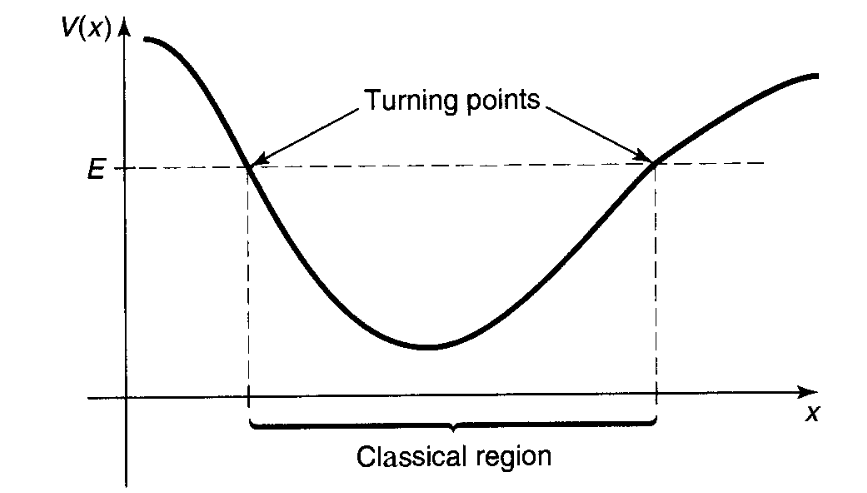
\includegraphics[width=0.4\linewidth]{image4.png}
\caption[skip=0pt]{\label{fig:4}\emph{Transmission through potential}}
\end{figure}
\begin{itemize}
    \item Now we can make the following ansatz. Since the wavefunction is a complex function it can be written in terms of a function that determines the amplitude $A(x)$ and a function that determine the phase $\phi(x)$. So:
\begin{bux}
    \begin{split}
        \psi(x) = A(x)e^{i\phi(x)}
    \end{split}
\end{bux}
both of these are real functions. We can then plug this into our Schr\"odinger equation \ref{eqn:4.4'}, resulting in:
\begin{bux}
    \begin{split}
        (A''+2iA'\phi'+i\phi''A-(\phi')^2A)e^{i\phi}) = -\frac{p^2}{\hbar^2}Ae^{i\phi}
    \end{split}
\end{bux}
This gives us two equations, one for the real and one for the imaginary components:
\begin{bux}
    \begin{split}
\label{eqn:4.7'}
        & A''-(\phi')^2A=-\frac{p^2}{\hbar^2}A \\
        & 2A'\phi'+\phi''A = 0
    \end{split}
\end{bux}
\item For the second equation we can notice we can write this as: $(\phi'A^2)=0\implies A^2\phi' = C^2$ or more simply:
\begin{bux}
    \begin{split}
        A = \frac{C}{\sqrt{|\phi'|}}
    \end{split}
\end{bux}
Where $C$ is a real constant. We take the absolute value of $\phi'$ here as we know our amplitude must be real and $\phi'<0$, just corresponds to the wave propagating to the left instead of to the right, this  symmetrically shouldn't make the amplitude become complex.  For the first equation in \ref{eqn:4.7'}, we do not have a general solution, so we make an approximation! We assume that across the region of interest, that our amplitude $A(x)$, varies slowly with respect to $\phi'^2$ and $p^2/\hbar^2$, i.e. we are deep in the potential well, so that the $A''$ term can be ignored. This reduce \ref{eqn:4.7'} to:
\begin{bux}
    \begin{split}
\label{eqn:4.9'}
      &  (\phi')^2 = \frac{p^2}{\hbar^2} \implies \frac{d\phi}{dx} = \pm \frac{p}{\hbar} \\
& \implies \phi(x) = \pm\frac{1}{\hbar}\int p(x)dx
    \end{split}
\end{bux}
Can ignore the constant added to this as it can be absorbed into $C$ (making it not real anymore) along with a $\hbar$, when we write out the full wavefunction:
\begin{bux}
    \begin{split}
\label{eqn:4.10'}
        \psi_{\rm WKB}(x) = \frac{C}{\sqrt{p}}e^{\pm\frac{i}{\hbar}\int p(x)dx}
    \end{split}
\end{bux}
The general solution will be a linear combination of the two $\pm$, terms. 

\item We can notice from this that $|\psi(x)|^2 = \frac{|C|^2}{p}$, i.e. the probability of finding a particle somewhere is inversely proportional to its classical momentum at that point, which is what we would expect, the particle doesn't spend long at places where it is moving rapidly, so it is less likely to be found there. 
\end{itemize}

\subsubsection{Quantisation condition}
\begin{itemize}
    \item If we have an infinite square well of length $a$, with some potential at the bottom that makes it "bumpy". We know then that our solution with the WKB approximation \ref{eqn:4.10'}, will take the following form in order to vanish at $x=0$ and $x=a$:
\begin{bux}
    \begin{split}
        \psi \simeq \frac{C}{\sqrt{p}}\sin(\phi(x))
    \end{split}
\end{bux}
With this we can obtain a quantisation condition from the requirement that $\phi(a)=n\pi$, which due to \ref{eqn:4.9'} is:
\begin{bux}
    \begin{split}
        \int_0^ap(x)dx = n\pi\hbar
    \end{split}
\end{bux}
This is our general \emph{quantisation condition}. 

\end{itemize}

\subsubsection{Quantum region}
\begin{itemize}
    \item We would like to extend this approximation to the quantum region. Specifically we mean for when the potential is far larger then the potential $V>>E$. This means our momentum is now complex so we can use a trick that we often use in the case of the square well. We can absorb the $i$ in the exponent so that \ref{eqn:4.10'} takes the form:
\begin{bux}
    \begin{split}
           \psi_{\rm WKB}(x) = \frac{C}{\sqrt{p}}e^{\pm\frac{1}{\hbar}\int |p(x)|dx}
    \end{split}
\end{bux}
Where now $|p(x)|= \sqrt{2m(V(x)-E)}$.
\end{itemize}

\subsubsection{Connection point}
\begin{itemize}
    \item We have demonstrated how the WKB approximation works for $V>>E$ and $E<<V$, but what if $E \sim V$. Then our approximations we have made before break down, as at the turning point when $E \sim V$ , $p\rightarrow 0  $ making our wavefunction blow up. This is not some feature of the wavefunction our approximation is simply failing here. What we need to fix this is a patching wavefunction $\psi_p$ that smoothing transitions between our classical and quantum region at this point. 

\item The simplest way to do this is to approximate the potential to be linear at the crossing point $V(x) = E+V'(0)x$.  This is nice as this is something we can solve the Schr\"odinger equation for analytically:
\begin{bux}
    \begin{split}
        -\frac{\hbar^2}{2m}&\frac{d^2\psi_p}{dx^2}+(E+V'(0)x)\psi_p) = E\psi_p \\
& \implies \frac{d^2\psi_p}{dx^2} = \alpha^3x\psi_p
    \end{split}
\end{bux}
Where $\alpha=\left(\frac{2mV'(0)}{\hbar^2}\right)^{1/3}$, then making the substitution $z=ax$, we arrive at a familiar equation:
\begin{bux}
    \begin{split}
        \frac{d^2\psi_p}{dz^2} = z\psi_p
    \end{split}
\end{bux}
This is the \emph{Airy equation}, whose solutions are special functions aptly named the \emph{Airy Functions} $\rm Ai(x)$ and $Bi(x)$. 

\item We should also note that with the above definitions we can write our momentum as $p(x) \simeq \sqrt{2m(E-E-V'(0)x)} = \hbar\alpha^{3/2}\sqrt{-x}$. This is useful later when we want to calculate the transmission probability. 
\end{itemize}










\subsubsection{Transmission coefficient} 
\begin{itemize}
    \item  We wish to calculate the transmission coefficient for a wave function incident on a section of potential of length $a$ that we have used the WKB approximation to obtain a wave function for. The situation described is shown in the below Figure \ref{fig:2}

\begin{figure}[H]
\centering
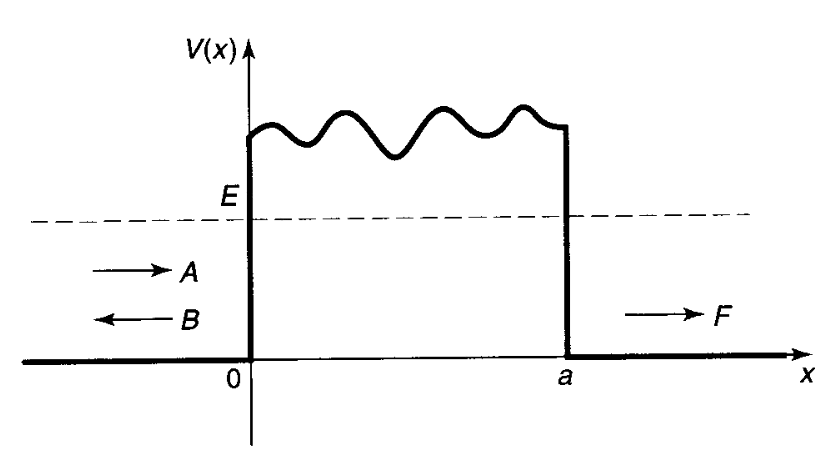
\includegraphics[width=0.4\linewidth]{image2.png}
\caption[skip=0pt]{\label{fig:2}\emph{Transmission through potential}}
\end{figure}

From the WKB approximation we have that the wave function for this potential is given by:
\begin{bux}
    \begin{split}
\label{eqn:4.3}
        \psi_{\rm WKB}(x) = \begin{cases}
           & \frac{1}{\sqrt{p(x)}}\left[Ae^{\frac{i}{\hbar}\int_x^0p(x')dx'}+Be^{-\frac{i}{\hbar}\int_x^0p(x')dx'}\right],~~~(x<0) \\
         & \frac{1}{\sqrt{|p(x)}|}\left[Ce^{\frac{1}{\hbar}\int^x_0|p(x')|dx'}+De^{-\frac{1}{\hbar}\int^x_0|p(x')|dx'}\right],~~~(0<x<a) \\
 & \frac{1}{\sqrt{p(x)}}\left[Fe^{\frac{i}{\hbar}\int^x_ap(x')dx'}\right],~~~(a<x)
        \end{cases}
    \end{split}
\end{bux}
The problem is we cannot just use continuity of the wavefunction or its derivatives to relate these coefficients, what we must do instead is use a patching wavefunction $\psi_p(x)$ , which can be shown to be given by (a linear combination of ) the Airy functions:
\begin{bux}
    \begin{split}
\label{eqn:4.4}
        \psi_p(x) = a\rm Ai(\alpha x) + b\rm Bi(\alpha x)
    \end{split}
\end{bux}
Where $\alpha \equiv \left(\frac{2mV'(0)}{\hbar^2}\right)^{1/3}$. Far from $0$ ($x>>0$), these two functions asymptotically behave like:
\begin{bux}
    \begin{split}
\label{eqn:4.5}
     &   \rm Ai(x) \simeq \frac{1}{2\sqrt{\pi}x^{1/4}}e^{-\frac{2}{3}x^{3/2}} \\
& \rm Bi(x) \simeq \frac{1}{\sqrt{\pi}x^{1/4}}e^{\frac{2}{3}x^{3/2}}
    \end{split}
\end{bux}
Using these we can write our patching wavefunction \ref{eqn:4.4} as:
\begin{bux}
    \begin{split}
\label{eqn:4.6}
        \psi_p(x) \simeq \frac{a}{2\sqrt{\pi}(\alpha x)^{1/4}}e^{-\frac{2}{3}(\alpha x)^{3/2}} + \frac{b}{\sqrt{\pi}(\alpha x)^{1/4}}e^{\frac{2}{3}(\alpha x)^{3/2}}
    \end{split}
\end{bux}
\item We also have at the overlap point ($x=0$) that $V(x) \simeq E + xV'(0) $, so $p(x) = \sqrt{2m(E-E-V'(0)x)} = \hbar \alpha^{3/2}\sqrt{-x}$.  From this we can easily calculate the power of the above wavefunctions: 
\begin{bux}
    \begin{split}
\label{eqn:4.7}
     &    \int_x^0\hbar \alpha^{3/2}\sqrt{-x'}dx' = \frac{2}{3}\hbar(-\alpha x)^{3/2},~~~x<0 \\
&  \int^x_0|\hbar \alpha^{3/2}\sqrt{-x'}|dx' = \frac{2}{3}\hbar(\alpha x)^{3/2},~~~x>0
    \end{split}
\end{bux}
Using these we can write our middle WKB wave function \ref{eqn:4.3} around the first overlap point ($x=0$), as:
\begin{bux}
    \begin{split}
\label{eqn:4.8}
          \psi_{\rm WKB}(x) = \frac{1}{\sqrt{\hbar}\alpha^{3/4}x^{1/4}}\left[Ce^{\frac{2}{3}(\alpha x)^{3/2}}+De^{-\frac{2}{3}(\alpha x)^{3/2}}\right],~~~(0<x<a)
    \end{split}
\end{bux}
Comparing these two wavefunctions \ref{eqn:4.6} and \ref{eqn:4.8}, we can see that:
\begin{bux}
    \begin{split}
\label{eqn:4.9}
        a = 2D\sqrt{\frac{\pi}{\alpha \hbar}},~~~b = C\sqrt{\frac{\pi}{\alpha \hbar}}
    \end{split}
\end{bux}
\item We also have that far from $0$ ($x<<0$), the Airy functions , behave like:
\begin{bux}
    \begin{split}
\label{eqn:4.10}
         &   \rm Ai(x) \simeq \frac{1}{\sqrt{\pi}(-x)^{1/4}}\rm sin\left[\frac{2}{3}(-x)^{3/2}+\frac{\pi}{4}\right] \\
& \rm Bi(x) \simeq -\frac{1}{\sqrt{\pi}(-x)^{1/4}}\rm cos\left[\frac{2}{3}(-x)^{3/2}+\frac{\pi}{4}\right]
    \end{split}
\end{bux}
Using these we can write our patching wavefunction \ref{eqn:4.4} as:
\begin{bux}
    \begin{split}
\label{eqn:4.11}
        \psi_p(x) &\simeq \frac{a}{\sqrt{\pi}(-\alpha x)^{1/4}}\rm sin\left[\frac{2}{3}(-\alpha x)^{3/2}+\frac{\pi}{4}\right] +-\frac{b}{\sqrt{\pi}(-\alpha x)^{1/4}}\rm cos\left[\frac{2}{3}(-\alpha x)^{3/2}+\frac{\pi}{4}\right] \\
& = \frac{1}{2\sqrt{\pi}(-\alpha x)^{1/4}}\left[(-ia+b)e^{i\frac{2}{3}(-\alpha x)^{3/2}}e^{i\pi/4}+(ia+b)e^{-i\frac{2}{3}(-\alpha x)^{3/2}}e^{-i\pi/4}\right]
    \end{split}
\end{bux}
\item Then for the Left WKB function we can use \ref{eqn:4.7}, to write \ref{eqn:4.3} as:
\begin{bux}
    \begin{split}
\label{eqn:4.12}
          \psi_{\rm WKB}(x) =
           &  \frac{1}{\sqrt{\hbar}\alpha^{3/4}(-x)^{1/4}}\left[Ae^{i\frac{2}{3}\hbar(-\alpha x)^{3/2}}+Be^{-i\frac{2}{3}\hbar(-\alpha x)^{3/2}}\right],~~~(x<0)
    \end{split}
\end{bux}
Comparing \ref{eqn:4.11} and \ref{eqn:4.12}, as we expect them to asymptotically become the same, we get the following relations:
\begin{bux}
    \begin{split}
        A = \sqrt{\frac{\hbar\alpha}{\pi}}\left(\frac{-ia+b}{2}\right)e^{i\pi/4},~~~B = \sqrt{\frac{\hbar\alpha}{\pi}}\left(\frac{ia+b}{2}\right)e^{-i\pi/4}
    \end{split}
\end{bux}
\item We can then compare these with the relations in \ref{eqn:4.9}, to obtain:
\begin{bux}
    \begin{split}
\label{eqn:4.14}
        A =\left(\frac{C}{2}-iD\right)e^{i\pi/4},~~~B=\left(\frac{C}{2}+iD\right)e^{-i\pi/4}
    \end{split}
\end{bux}
\item We then have to just repeat this procedure for the second overlapping point ($x=a$),  For this we take our middle WKB wavefunction from \ref{eqn:4.3} and write it in the following way:
\begin{bux}
    \begin{split}
       \psi_{\rm WKB} =  \frac{1}{\sqrt{|p(x)}|}\left[Ce^{\frac{1}{\hbar}\left(\int_0^a|p(x')|dx'-\int_x^a|p(x')|dx'\right)}+De^{-\frac{1}{\hbar}\left(\int_0^a|p(x')|dx'-\int_x^a|p(x')|dx'\right)}\right]
    \end{split}
\end{bux}
Then if we call $\gamma \equiv \frac{1}{\hbar}\int_0^a|p(x')|dx'$, and relabel, $C'\equiv De^{-\gamma}$ , $D'\equiv Ce^{\gamma}$, then shift $x=a$ to be the origin,  we have that:
\begin{bux}
    \begin{split}
\label{eqn:4.16}
         \psi_{\rm WKB}(x) = \begin{cases}
         & \frac{1}{\sqrt{|p(x)}|}\left[C'e^{\frac{1}{\hbar}\int_x^0|p(x')|dx'}+D'e^{-\frac{1}{\hbar}\int_x^0|p(x')|dx'}\right],~~~(0<x<a) \\
 & \frac{1}{\sqrt{p(x)}}\left[Fe^{\frac{i}{\hbar}\int^x_0p(x')dx'}\right],~~~(a<x)
        \end{cases}
    \end{split}
\end{bux}
At the overlap point ($x=0$) we now have that that $V(x) \simeq E - xV'(0) $, so $p(x) = \sqrt{2m(E-E+V'(0)x)} = \hbar \alpha^{3/2}\sqrt{x}$ ($\alpha\equiv \left(\frac{2m|V'(0)|}{\hbar^2}\right)^{1/3}$ ).  From this we can easily calculate the power of the above wavefunctions: 
\begin{bux}
    \begin{split}
\label{eqn:4.17}
     &    \int_x^0|\hbar \alpha^{3/2}\sqrt{x'}|dx' = \frac{2}{3}\hbar(-\alpha x)^{3/2},~~~x<0 \\
&  \int^x_0\hbar \alpha^{3/2}\sqrt{x'}dx' = \frac{2}{3}\hbar(\alpha x)^{3/2},~~~x>0
    \end{split}
\end{bux}
This means our middle WKB wavefunctions in \ref{eqn:4.16} take the form:
\begin{bux}
    \begin{split}
\label{eqn:4.18}
         \psi_{\rm WKB}(x) = 
         & \frac{1}{\sqrt{\hbar^{1/2}}\alpha^{3/4}(-x)^{1/4}}\left[C'e^{\frac{2}{3}(-\alpha x)^{3/2}}+D'e^{-\frac{2}{3}\hbar(-\alpha x)^{3/2}}\right],~~~(0<x<a)
    \end{split}
\end{bux}
\item Our patching for his point is then also around $x=0$, as we have moved the origin, but this time the Airy function is sloping down so:
\begin{bux}
    \begin{split}
        \psi_p(x) = a\rm Ai(-\alpha x) + b\rm Bi(-\alpha x)
    \end{split}
\end{bux}
Close to our overlap point ($x=0$) ,for $x<<0$ we have that these Airy functions behave like \ref{eqn:4.5} (as if we swap $x \rightarrow -x$ then $x>>0$ and our Airy functions are the same as \ref{eqn:4.5}), so:
\begin{bux}
    \begin{split}
\label{eqn:4.20}
        \psi_p(x) \simeq \frac{a}{2\sqrt{\pi}(-\alpha x)^{1/4}}e^{-\frac{2}{3}(-\alpha x)^{3/2}}+\frac{b}{\sqrt{\pi}(-\alpha x)^{1/4}}e^{\frac{2}{3}(-\alpha x)^{3/2}}
    \end{split}
\end{bux}
\item We can then compare these two wavefunctions \ref{eqn:4.18} and \ref{eqn:4.20}, as they must become the same for $x<<0$, comparing them allows us to read off:
\begin{bux}
    \begin{split}
\label{eqn:4.21}
        a=2\sqrt{\frac{\pi}{\hbar\alpha}}D',~~~b=\sqrt{\frac{\pi}{\hbar\alpha}}C'
    \end{split}
\end{bux}
\item Finally we just have to relate our overlap function $\psi_p$, to our right WKB wavefunction in \ref{eqn:4.16}, which we can write, using \ref{eqn:4.17} as:
\begin{bux}
    \begin{split}
\label{eqn:4.22}
      \psi_{\rm WKB} \simeq  \frac{1}{\sqrt{	\hbar}\alpha^{3/4}x^{1/4}}\left[Fe^{i\frac{2}{3}(\alpha x)^{3/2}}\right]
    \end{split}
\end{bux}
In this region our overlap function of Airy functions will behave using the $x>>0$ limits, given by \ref{eqn:4.10} (as the argument of our airy functions are negative):
\begin{bux}
    \begin{split}
\label{eqn:4.23}
        \psi_p(x) &\simeq \frac{a}{\sqrt{\pi}(\alpha x)^{1/4}}\rm sin\left[\frac{2}{3}(\alpha x)^{3/2}+\frac{\pi}{4}\right] +-\frac{b}{\sqrt{\pi}(\alpha x)^{1/4}}\rm cos\left[\frac{2}{3}(\alpha x)^{3/2}+\frac{\pi}{4}\right] \\
& = \frac{1}{2\sqrt{\pi}(\alpha x)^{1/4}}\left[(-ia+b)e^{i\frac{2}{3}(\alpha x)^{3/2}}e^{i\pi/4}+(ia+b)e^{-i\frac{2}{3}(\alpha x)^{3/2}}e^{-i\pi/4}\right]
    \end{split}
\end{bux}
Comparing \ref{eqn:4.22} and \ref{eqn:4.23}, we see that:
\begin{bux}
    \begin{split}
       &  ia+b= 0 ,~~~F = \sqrt{\frac{\hbar\alpha}{\pi}}\left(\frac{-ia+b}{2}\right)e^{i\pi/4} \\ 
& \implies b = \sqrt{\frac{\pi}{\hbar\alpha}}e^{-i\pi/4}F,~~~a=i\sqrt{\frac{\pi}{\hbar\alpha}}e^{-i\pi/4}F
    \end{split}
\end{bux}
Then we can use relations \ref{eqn:4.21} to write:
\begin{bux}
    \begin{split}
        De^{-\gamma} =C' = e^{-i\pi/4}F,~~~Ce^{\gamma} =D' = \frac{i}{2}e^{-i\pi/4}F,
    \end{split}
\end{bux}
Which we can then plug into the relations \ref{eqn:4.14} to get:
\begin{bux}
    \begin{split}
        A =\left(\frac{C}{2}-iD\right)= \left(\frac{i}{4}e^{-\gamma}e^{-i\pi/4}F-ie^{\gamma}e^{-i\pi/4}F\right)e^{i\pi/4} = i\left(\frac{e^{-\gamma}}{4}-e^{\gamma}\right)F
    \end{split}
\end{bux}
This finally gives us our expression for the transmission coefficient! :
\begin{bux}
    \begin{split}
        T \equiv |\frac{F}{A}|^2 = \frac{1}{(e^{\gamma}-\frac{e^{-\gamma}}{4})^2} = \frac{e^{-2\gamma}}{(1-(e^{-\gamma}/2)^2)^2}
    \end{split}
\end{bux}
To first order in $\gamma\equiv \frac{1}{\hbar}\int_0^a|p(x')|dx'$, i.e. assuming $a$, the length of our potential is large, reduces to the result we want:
\begin{bux}
    \begin{split}
        T\simeq e^{-\frac{2}{\hbar} \int_0^a|p(x')|dx'}
    \end{split}
\end{bux}


\end{itemize}
\newpage
\section{Time Dependant perturbation theory}
\begin{itemize}
    \item With Time dependence comes the time dependent Schr\"odinger equation: 
\begin{bux}
    \begin{split}
        \hat{H}\ket{\Psi} = i\hbar \frac{\partial}{\partial t}\ket{\Psi}
    \end{split}
\end{bux}
This can be solved with the separation of variables $\ket{\Psi(\textbf{r},t)} = e^{-iEt/\hbar}\ket{\psi(\textbf{r})}$ , where $\ket{\psi(\textbf{r})}$ satisfies TISE:
\begin{bux}
    \begin{split}
        \hat{H}\ket{\psi} = E\ket{\psi}
    \end{split}
\end{bux}
\item Since the time dependence is carried by the $e^{iEt/\hbar}$, the probability $|\braket{\psi|\psi}|^2$ is still constant in time. More interesting time dependent functions can be obtained by taking linear combinations of these states:
\begin{bux}
    \begin{split}
        \ket{\tilde{\Psi}(\textbf{r},t)} = \sum_nc_ne^{-iE_nt/\hbar}\ket{\psi_n(\textbf{r})}
    \end{split}
\end{bux}
But even then these coefficients are not dependant on time, if we want to allow for transitions or quantum jumps, between different energy levels we need to introduce a time dependant potential. This is a difficult problem to solve, but if the time dependant addition to the Hamiltonian is small then we may use perturbation theory to obtain results to certain order. We wil ldo this in one dimension but the results are easily genralisable. 
 

\end{itemize}

\subsection{First order correction}
\begin{itemize}
    \item With the addition of a small time dependant potential are Hamiltonian now takes the form: 
\begin{bux}
    \begin{split}
        \hat{H} = \hat{H}^{(0)}+gV^{(1)}(x,t)
    \end{split}
\end{bux}
Where $g$ is a small parameter. Our wavefunctions now take the form:
\begin{bux}
    \begin{split}
        \ket{\psi(t)} = \sum_nc_n(t)e^{-iE_nt/\hbar}\ket{\psi_n}
    \end{split}
\end{bux}
Notability are coefficients are now functions of time. We will then expand these coefficients perturbatively:
\begin{bux}
    \begin{split}
        c_n(t) = c_n^{(0)}+gc_n^{(1)}(t)+g^2c_n^{(2)}(t)+\mathcal{O}(g^3)
    \end{split}
\end{bux}
Note that the $0$th order terms have no time dependence as if we turn the perturbation off we don't expect the coefficients to be time dependant 

\item We now can plug our wavefunction into the time dependant Schr\"odinger equation to first order in $g$:
\begin{bux}
    \begin{split}
         (\hat{H}^{(0)}+gV^{(1)})&\left[\sum_n(c_n^{(0)}+gc_n^{(1)}(t))e^{-iE_nt/\hbar}\ket{\psi_n}\right] \\
 = i\hbar\frac{\partial}{\partial t}&\left[\sum_n(c_n^{(0)}+gc_n^{(1)}(t))e^{-iE_nt/\hbar}\ket{\psi_n}\right]
    \end{split}
\end{bux}
Comparing the terms that don't have $g$, when we expand we find:
\begin{bux}
    \begin{split}
        \sum_nE_nc_n^{(0)}e^{-iE_nt/\hbar}\ket{\psi_n}= i\hbar \sum_n(-i\frac{E_n}{\hbar})c_n^{(0)}e^{-iE_nt/\hbar}\ket{\psi_n}
    \end{split}
\end{bux}
So they cancel from both sides as expected. Now for the terms that are linear in $g$, we find:
\begin{bux}
    \begin{split}
      &   \sum_n\left[\hat{H}^{(0)}c_n^{(1)}(t)\ket{\psi_n}e^{-iE_nt/\hbar}+\hat{V}^{(1)}c_n^{(0)}(t)\ket{\psi_n}e^{-iE_nt/\hbar}\right] \\
&~~~~~~~~~~~~~~= i\hbar\sum_n\left[\frac{dc_n^{(1)}}{dt}-i\frac{E_n}{\hbar}c_n^{(1)}\right]\ket{\psi_n}e^{-iE_nt\hbar}
    \end{split}
\end{bux}
The first term on the LS and the last term on the RHS cancel as $\hat{H}^{(0)}\ket{\psi_n}=E_n\ket{\psi_n}$. This leaves us with:
\begin{bux}
    \begin{split}
         &     \sum_n\left[\hat{V}^{(1)}c_n^{(0)}(t)\ket{\psi_n}e^{-iE_nt/\hbar}\right]= i\hbar\sum_n\left[\frac{dc_n^{(1)}}{dt}\right]\ket{\psi_n}e^{-iE_nt\hbar} \\ 
& \implies \frac{dc_k^{(1)}}{dt} = -\frac{i}{\hbar}\sum_n\bra{\psi_k}V^{(1)}\ket{\psi_n}c_k^{(0)}e^{-i(E_n-E_k)t/\hbar}
    \end{split}
\end{bux}
Where in the last step we have acted on the left with $\bra{\psi_k}$.

\item Similarly the result for second order in $g$ can also be found with the result being:
\begin{bux}
    \begin{split}
      \frac{dc_k^{(2)}}{dt} =- \frac{i}{\hbar}\sum_n\bra{\psi_k}V^{(1)}\ket{\psi_n}c_k^{(1)}e^{-i(E_n-E_k)t/\hbar}
    \end{split}
\end{bux}
\end{itemize}


\newpage 
\section{The Path Integral}
\begin{itemize}
    \item The goal here is to motivate and derive the path integral in one-dimension.  If we have a single particle in a position eigenstate $\ket{x}$ at time $t$, we can write this as one ket $\ket{x ,t}$, now given the knowledge that the particle is in this state we would like to know what is the probability of finding the particle in some other state $\ket{x'}$ at time $t'$, this we can write as $\ket{x',t'}$.  The time dependence of these states can be easily dealt with by recalling that if the Hamiltonian governing our system is time independent then time evolution of a state is governed by the time evolution operator, i.e. :
\begin{bux}
    \begin{split}
       &  \ket{\psi(t)} = e^{\frac{i}{\hbar}\hat{H}t}\ket{\psi(t=0)} \\
& \implies \ket{x,t} =  e^{\frac{i}{\hbar}\hat{H}t}\ket{x} \\
 \implies &\bra{x',t'} =  \left(e^{\frac{i}{\hbar}\hat{H}t'}\ket{x'}\right)^{\ast} = \bra{x'}e^{-\frac{i}{\hbar}\hat{H}t'}
    \end{split}
\end{bux}
Now the probability that the particle initially in state $\ket{x,t}$, will end up in state $\ket{x',t'}$, is just the square of the final ket acting on the initial ket, i.e. $P(x',t') =|\braket{x',t'|x,t}|^2$. This quantity that is being squared can be expressed in terms of the Hamiltonian, using our time evolution operator as:
\begin{bux}
    \begin{split}
        \braket{x',t'|x,t} = \bra{x'}e^{-\frac{i}{\hbar}\hat{H}(t'-t)}\ket{x}
    \end{split}
\end{bux}
\item From now on we will call this quantity the propagator, as it is related to the the probability of a the particle propagating  to the new state. To calculate the form of this propagator, we need to take into account all possible ways a particle can continuously move from $\ket{x}$ to $\ket{x'}$. This seems a little daunting so to make it easier we can simplify the problem by discretizing time. Dividing the time interval $t'-t$, into $N$ steps of length $\Delta t = \frac{(t'-t)}{N}$. See the figure below \ref{fig:3}:
\begin{figure}[H]
\centering
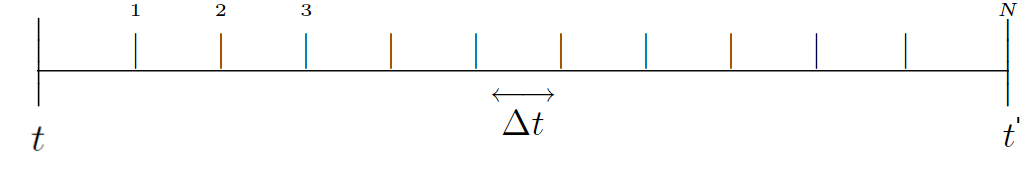
\includegraphics[width=0.7\linewidth]{image3.png}
\caption[skip=0pt]{\label{fig:3}\emph{Separating time into $N$ time steps of length $\Delta t$}}
\end{figure}
With this change our propagator takes the following form:
\begin{bux}
    \begin{split}
\label{eqn:5.3}
        \braket{x',t'|x,t}=\bra{x'}\left(e^{-\frac{i}{\hbar}\hat{H}\Delta t}\right)^N\ket{x}
    \end{split}
\end{bux}
\item The next step is definitely a trick, we are going to stick an identity $\mathbb{I}$ between each of the exponential terms here. The specific form of the identity we are going to stick in is the completeness relation of the  position kets, that is that:
\begin{bux}
    \begin{split}
        \mathbb{I} = \int dx\ket{x}\bra{x}
    \end{split}
\end{bux}
In one dimension we would be integrating over all of $\mathcal{R}$, so the bounds on this integral would go from $-\infty$, to $\infty$, but for simplicity we can just leave this as a definite integral, said to be over all $\ket{x}$. We then insert this identity $N-1$ times between the $N$ exponential terms in \ref{eqn:5.3}:
\begin{bux}
    \begin{split}
\label{eqn:5.5}
         & \braket{x',t'|x,t}  =\bra{x'}\left(e^{-\frac{i}{\hbar}\hat{H}\Delta t}\right)\mathbb{I}\left(e^{-\frac{i}{\hbar}\hat{H}\Delta t}\right)\mathbb{I}\cdot\cdot\cdot\mathbb{I}\left(e^{-\frac{i}{\hbar}\hat{H}\Delta t}\right)\ket{x} \\
  = \int dx_1 &\cdot\cdot\cdot  dx_{N-1}\bra{x'}e^{-\frac{i}{\hbar}\hat{H}\Delta t}\ket{x_{N-1}}\bra{x_{N-1}}e^{-\frac{i}{\hbar}\hat{H}\Delta t}\ket{x_{N-2}} \cdot\cdot\cdot \bra{x_{1}}e^{-\frac{i}{\hbar}\hat{H}\Delta t}\ket{x}
    \end{split}
\end{bux}
\item The next task will be to then see if we can calculate this individual propagators $\bra{x_i}e^{-\frac{i}{\hbar}\hat{H}\Delta t}\ket{x_j}$, which are basically just the propagators for a single time step. For a single particle the Hamiltonian takes the form, $\hat{H} = \frac{\hat{P}^2}{2m}+\hat{V}$, where $\hat{V}$ is some general potential, which is only a function of position, not momentum.  There is then a slight issue with separating these terms from each other in the exponential, since we know for operators that:
\begin{bux}
    \begin{split}
        e^{\hat{A} +\hat{B}} = e^{\hat{A}}e^{\hat{B}}e^{[\hat{A},\hat{B}]}
    \end{split}
\end{bux}
But since for the operators in the our exponential $-\frac{i}{\hbar}\hat{H}\Delta t= -\frac{i}{\hbar}\left(\frac{\hat{P}^2}{2m}+\hat{V}\right)\Delta t \implies [-\frac{i}{\hbar}\frac{\hat{P}^2}{2m}\Delta t,-\frac{i}{\hbar}\hat{V}\Delta t] =\frac{1}{\hbar^2}\frac{\hat{P}^2}{2m}\hat{V}\Delta t^2-\frac{1}{\hbar^2}\hat{V}\frac{\hat{P}^2}{2m}\Delta t^2 = \mathcal{O}(\Delta t^2)$ , so if we consider $\Delta t$, to be a very small parameter, and ignore terms of  $\mathcal{O}(\Delta t^2)$, then we have no issue splitting up our exponential terms. This means we can write a single step propagator as:
\begin{bux}
    \begin{split}
         \bra{x_i}e^{-\frac{i}{\hbar}\hat{H}\Delta t}\ket{x_j} \simeq \bra{x_i}e^{-\frac{i}{\hbar}\frac{\hat{P}^2}{2m}\Delta t}e^{-\frac{i}{\hbar}\hat{V}\Delta t}\ket{x_j}
    \end{split}
\end{bux}
Now we can deal with the potential term first, by remembering that since it is just a function of position, it will act on the position eigenstate $\ket{x_j}$ via: $\hat{V}\ket{x} = V(x_j)\ket{x_j}$, this is because we can write $\hat{V}$ as a taylor expansion in $\hat{X}$, the position operator, $\hat{V} = \sum_{n=0}^{\infty}c_n\hat{X}^n$, so that $\hat{V}\ket{x_j} = \sum_{n=0}^{\infty}c_n\hat{X}^n\ket{x_j} =\sum_{n=0}^{\infty}c_nx_j^n\ket{x_j} =V(x_j)\ket{x_j}$. Then seeing as the exponential cal also be taylor expanded we get that:
\begin{bux}
    \begin{split}
        e^{-\frac{i}{\hbar}\hat{V}\Delta t}\ket{x_j} = \sum_{n=0}^{\infty}\frac{(-\frac{i}{\hbar}\hat{V}\Delta t)^n}{n!}\ket{x_j} = \sum_{n=0}^{\infty}\frac{(-\frac{i}{\hbar}V(x_j)\Delta t)^n}{n!}\ket{x_j} =  e^{-\frac{i}{\hbar}V(x_j)\Delta t}\ket{x_j}
    \end{split}
\end{bux}
So our one step propagator is now:
\begin{bux}
    \begin{split}
         \bra{x_i}e^{-\frac{i}{\hbar}\hat{H}\Delta t}\ket{x_j} = \bra{x_i}e^{-\frac{i}{\hbar}\frac{\hat{P}^2}{2m}\Delta t}e^{-\frac{i}{\hbar}V(x_j)\Delta t}\ket{x_j}
    \end{split}
\end{bux}
Now we cant say how $\hat{P}$, will act on $\ket{x_j}$, with out knowing the explicit form of $\ket{x_j}$, but to get around this we can insert another identity in between the exponential containing $\hat{P}$ and the ket $\ket{x_j}$, this time this identity will be the completeness relation for the momentum kets, which takes the form:
\begin{bux}
    \begin{split}
        \mathbb{I} = \int_{-\infty}^{\infty} dp \ket{p}\bra{p}
    \end{split}
\end{bux}
We have the bounds on the integral here as we will need to carry out this integral. This means we can write:
\begin{bux}
    \begin{split}
        \bra{x_i}e^{-\frac{i}{\hbar}\frac{\hat{P}^2}{2m}\Delta t}\mathbb{I}e^{-\frac{i}{\hbar}V(x_j)\Delta t}\ket{x_j} = \int_{-\infty}^{\infty} dp  \bra{x_i}e^{-\frac{i}{\hbar}\frac{\hat{P}^2}{2m}\Delta t}\ket{p}e^{-\frac{i}{\hbar}V(x_j)\Delta t}\braket{p|x_j}
    \end{split}
\end{bux}
In the same manor as the potential operator acted on the kets $\ket{x}$, the momentum operator acts on the kets $\ket{p}$ , via $\hat{P}\ket{p}=p\ket{p}$, so we can see that with the same procedure as above our propagator becomes:
\begin{bux}
    \begin{split}
          \bra{x_i}e^{-\frac{i}{\hbar}\hat{H}\Delta t}\ket{x_j} = \int_{-\infty}^{\infty} dp  \braket{x_i|p}e^{-\frac{i}{\hbar}\frac{p^2}{2m}\Delta t}e^{-\frac{i}{\hbar}V(x_j)\Delta t}\braket{p|x_j}
    \end{split}
\end{bux}
All that is left is to calculate $\braket{x_i|p}$ and $\braket{p|x_j}$. To do this we can look at the Fourier transforms of the position kets into the momentum space and visa versa. These take the form:
\begin{bux}
    \begin{split}
        & \ket{x} = \frac{1}{\sqrt{2\pi \hbar}}\int d \tilde{p} e^{-\frac{i\tilde{p}x}{\hbar}}\ket{\tilde p} \\
 & \ket{p} = \frac{1}{\sqrt{2\pi \hbar}}\int d \tilde{x} e^{\frac{ip\tilde{x}}{\hbar}}\ket{\tilde x} \\
& \implies \braket{x_i|p} = \frac{1}{\sqrt{2\pi \hbar}}e^{\frac{ipx_i}{\hbar}} \\
& \implies \braket{p|x_j} = \frac{1}{\sqrt{2\pi \hbar}}e^{-\frac{ipx_j}{\hbar}}
    \end{split}
\end{bux}
This then means that:
\begin{bux}
    \begin{split}
         \bra{x_i}e^{-\frac{i}{\hbar}\hat{H}\Delta t}\ket{x_j} = \frac{1}{2\pi \hbar}\int_{-\infty}^{\infty} dp  e^{\frac{i}{\hbar}p(x_i-x_j)}e^{-\frac{i}{\hbar}(\frac{p^2}{2m}+V(x_j))\Delta t}
    \end{split}
\end{bux}
This integral can be turned into a Gaussian integral if we complete the square in the exponent. This can be done as follows: 
\begin{bux}
    \begin{split}
     &    p(x_i-x_j)-[\frac{p^2}{2m}+V(x_j)]\Delta t = -\frac{\Delta t}{2m}\left[p^2-\frac{2m}{\Delta t}p(x_i-x_j)\right] -V(x_j)\Delta t\\ 
& = -\frac{\Delta t}{2m}\left[p-\frac{m}{\Delta t}(x_i-x_j)\right]^2-V(x_j)\Delta t+\frac{m}{2\Delta t}(x_i-x_j)^2
    \end{split}
\end{bux}
So we can write our integral as:
\begin{bux}
    \begin{split}
       & \bra{x_i}e^{-\frac{i}{\hbar}\hat{H}\Delta t}\ket{x_j}  = \frac{e^{\frac{i}{\hbar}\left(\frac{m}{2\Delta t}(x_i-x_j)^2-V(x_j)\Delta t\right)}}{2\pi \hbar}\int_{-\infty}^{\infty} dpe^{-\frac{i}{\hbar}\frac{\Delta t}{2m}\left[p-\frac{m}{\Delta t}(x_i-x_j)\right]^2} \\
 = &\frac{e^{\frac{i}{\hbar}\left(\frac{m}{2\Delta t}(x_i-x_j)^2-V(x_j)\Delta t\right)}}{2\pi \hbar}\sqrt{\frac{2m\hbar}{i\Delta t}}\int_{-\infty}^{\infty} due^{-u^2},~~~(u=\sqrt{\frac{i\Delta t}{2m\hbar}}[p-\frac{m}{\Delta t}(x_i-x_j)]) \\
&~~~~~~~~~~~~~~~~~~~~~~~~~~ = \sqrt{\frac{m}{2\pi\hbar i\Delta t}}e^{\frac{i}{\hbar}\left(\frac{m}{2}(\frac{x_i-x_j}{\Delta t})^2\Delta t-V(x_j)\Delta t\right)}
    \end{split}
\end{bux}
Where here the integral just evaluated to $\sqrt{\pi}$. We can now consider how each term in the integral in \ref{eqn:5.5} takes the above form, there are $N$, such terms so plugging in we find: 
\end{itemize}
\begin{bux}
    \begin{split}
        \braket{x',t'|x,t} = \int dx_1 \cdot\cdot\cdot  dx_{N-1}\left(\frac{m}{2\pi\hbar i\Delta t}\right)^{N/2}\rm exp\left[\frac{i}{\hbar}\sum_{i=0}^{N-1}\left(\frac{m}{2}(\frac{x_i-x_{i+1}}{\Delta t})^2-V(x_{i+1})\right)\Delta t\right]
    \end{split}
\end{bux}
\begin{itemize}
 \item  Here for simplicity, we have relabeled $x' \rightarrow x_N$ and $x\rightarrow x_0$, so that the exponents can be written in terms of a single sum. These labelings also make sense as they are the start and end points of the path. All that is left to do with this is to recognise that $\frac{x_i-x_{i+1}}{\Delta t}$, is a single step divided by the time taken, thus, when we take the limit as $\Delta t \rightarrow dt$, then this quantity becomes the velocity $v$. With this we can see that first term in the exponential is $\frac{1}{2}mv^2$, i.e. our classical Kinetic energy, and $V$ is just our potential. This quantity of the Kinetic minus the potential energy is familiar to us! It is just the classical Lagrangian $L$! Furthermore, as we take the limit $\Delta t \rightarrow dt$, then $N\rightarrow \infty$ and the sum in the exponent becomes an integral wrt time. But the integral of the Lagrangian with respect to time is another quantity we know from classical mechanics, this is just the classical action $S[x(t)]$! Putting all this together and relabeling our nasty $dx_1 \cdot\cdot\cdot  dx_{N-1}\left(\frac{m}{2\pi\hbar i\Delta t}\right)^{N/2} \rightarrow \mathcal{D}x(t)$, results in the path Integral: 
\begin{bux}
    \begin{split}
         \braket{x',t'|x,t}  = \int\mathcal{D}x(t)e^{\frac{iS[x(t)]}{\hbar}}
    \end{split}
\end{bux}
\item Finally a beautiful observation from this path Integral is how it can explain why in classical mechanics that the action is minimised along the path the particle takes. This is outlined by the following argument by Dirac!: 
\small
\vspace{5mm}


\emph{...we see that the integrand in (11) must be of the form $e^{\frac{iS}{\hbar}}$, where $S$ is a function of \textit{q}\textsubscript{\textit{T}}, \textit{q}\textsubscript{1}, \textit{q}\textsubscript{2}, … \textit{q}\textsubscript{\textit{m}}, \textit{q}\textsubscript{\textit{t}}, which remains finite as $\hbar$   tends to zero. Let us now picture one of the intermediate \textit{q}s, say \textit{q\textsubscript{k}}, as varying continuously while the other ones are fixed. Owing to the smallness of \textit{h}, we shall then in general have $S/\hbar$ varying extremely rapidly. This means that $e^{\frac{iS}{\hbar}}$ will vary periodically with a very high frequency about the value zero, as a result of which its integral will be practically zero. The only important part in the domain of integration of \textit{q\textsubscript{k}} is thus that for which a comparatively large variation in \textit{q\textsubscript{k}} produces only a very small variation in \textit{F}. This part is the neighbourhood of a point for which $S$ is stationary with respect to small variations in \textit{q\textsubscript{k}}. We can apply this argument to each of the variables of integration ... and obtain the result that the only important part in the domain of integration is that for which $S$ is stationary for small variations in all intermediate \textit{q}s. ... We see that \textit{F} has for its classical analogue $\int_T^tLdt$, which is just the action function, which classical mechanics requires to be stationary for small variations in all the intermediate \textit{q}s. This shows the way in which equation (11) goes over into classical results when \textit{h} becomes extremely small. ~~~~~~~~~~~~~~~
-Dirac (1933), pg 69}


\end{itemize}













\end{document}
